\documentclass{book}

\usepackage{/home/mccoid/LaTeX/preamble}
%\usepackage{C:/Users/conmc/Documents/LaTeX/preamble}

\setcounter{MaxMatrixCols}{20}

\begin{document}

\chapter{Preconditioning Newton's method}

Given an equation $f(x) = 0$, we attempt to precondition Newton's method by finding a fixed point iteration of this equation, $g(x) = x$, then solving $g(x) - x = 0$ using Newton's method:
\begin{equation}
p_{n+1} = p_n - \frac{g(p_n) - p_n}{g'(p_n) - 1} .
\end{equation}
This equates to finding a new function ($f_1(x)$) that shares at least one root with $f(x)$.

Ideal qualities of functions to be solved:
\begin{itemize}
\item $f'(x*) \neq 0$ (for accuracy purposes)
\item both $f(x)$ and $f'(x)$ are easy to compute (for efficiency purposes)
\item $f(x)$ should allow for a wide range of initial guesses (basin of attraction) - this should relate to the region of monotonicity surrounding the root
\item $f''(x)$ should be small or zero (for faster convergence)
\end{itemize}

The iteration above can be rewritten as
\begin{equation*}
p_{n+1} = \frac{p_n g'(p_n) - g(p_n)}{g'(p_n) - 1} .
\end{equation*}
The error behaves as
\begin{equation*}
\norm{p^* - p_{n+1}} = \norm{ \sum_{k=2}^\infty \frac{ (p^* - p_n)^k g^{(k)}(p_n) }{(1 - g'(p_n)) k!} }
\end{equation*}
which is the same as Newton's method using $f(x) = x - g(x)$.
It can alternatively be written in terms of the unknown variable $\xi \in [x^*,x_n]$:
\begin{equation*}
\norm{p^* - p_{n+1}} = \frac{1}{2} \norm{p^* - p_n}^2 \norm{ \frac{ g''(\xi) }{1 - g'(p_n)} } .
\end{equation*}

Suppose we consider the preconditioned Newton's method as a fixed point iteration.
Then we would like the iterate to satisfy the conditions of the fixed point iteration theorem.
In particular, we would like the magnitude of the derivative of the iterate to be less than one near the root:
\begin{equation*}
\abs{ g''(p) \frac{g(p) - p}{\left ( g'(p) - 1 \right)^2} } < 1 .
\end{equation*}
Thus, we require that either $g''(p)$ or $g(p) - p$ is very small or $g'(p) - 1$ is very large.

Take as an example $g(x) = -\log(x)$.
For $p$ near the root $g(p) - p$ is very small.
For $p$ away from the root $g''(p)$ is very small.
The only issue is when $g'(p) = 1$, in which case there is a singularity.
This occurs for $p=-1$, and is a point from which the iterate cannot converge.

\section{Experiments}

\subsection{Experiment 1}

Our first trials are run using the function
\begin{equation}
f(x) = x e^x - 1 = 0 .
\end{equation}
Known as the Lambert W function, the roots of this function are well known and can be called in Matlab using \texttt{lambertw(branch,1)}.
The function has an infinite number of branches.

We compare using Newton's method on $f(x)$ with using Newton's method on the rearranged fixed point iteration
\begin{equation*}
g(x) = \log(x) + x - i k 2 \pi ,
\end{equation*}
where $k$ represents the branch of the function sought.
We make the following notes on their differences:
\begin{itemize}
\item $g(x)$ (and all its derivatives) has a singularity at $x=0$
\item $g'(x)$ and $f'(x)$ have roots at $x=-1$
\item all derivatives of $f(x)$ have roots, which gradually move towards $-\infty$
\item all other derivatives of $g(x)$ have no roots
\item the limit of all the derivatives of $g(x)$ as $x$ approaches $\pm \infty$ are finite (and zero except for $g'(x)$)
\item $\lim_{x \to -\infty} f^{(n)}(x) = 0 \ \forall n\geq 1$ and $\lim_{x \to \infty} f^{(n)}(x) = \infty \ \forall n \geq 0$
\end{itemize}

Using $g(x)$ shows significant improvement over $f(x)$.
Not only does the basin of attraction encompass essentially the entire complex plane (minus the points $x=-1, 0, e$ where the iteration has a singularity, fixed point and root, respectively) but the number of iterations required to reach a given tolerance drops for the majority of the original basin.
Moreover, $g(x)$ allows for great control on which root of $f(x)$ we seek.
Choosing different $k$ will allow us to converge to a different root of the function.
It appears any branch may be selected with a high degree of accuracy resulting.

Testing using $h(x) = x - e^{-x}$ shows an intermediate preconditioner.
It widens the basin of attraction, albeit with several remaining fractal areas and 'off-roots' where Newton's method refuses to converge.
The function $h(x)$ has the following properties:
\begin{itemize}
\item the limit of $h(x)$ as $x$ approaches either infinity is infinite
\item the same limits for the derivatives of $h(x)$ are finite for $+ \infty$ and infinite for $-\infty$
\item $h'(x)$ has a root at $x=0$, subsequent derivatives are everywhere non-zero
\end{itemize}

\begin{figure}
	\begin{subfigure}{0.5\textwidth}
		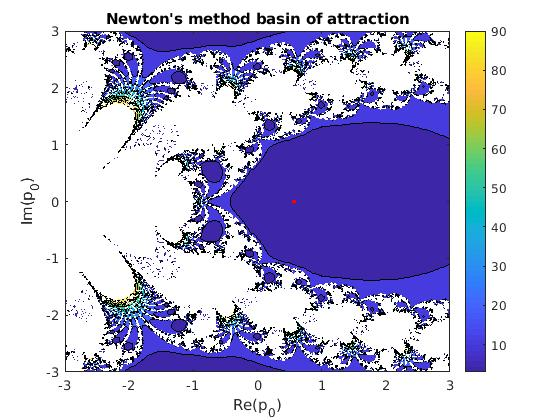
\includegraphics[width=\textwidth]{exp1_01.jpg}
	\end{subfigure}
	\begin{subfigure}{0.5\textwidth}
		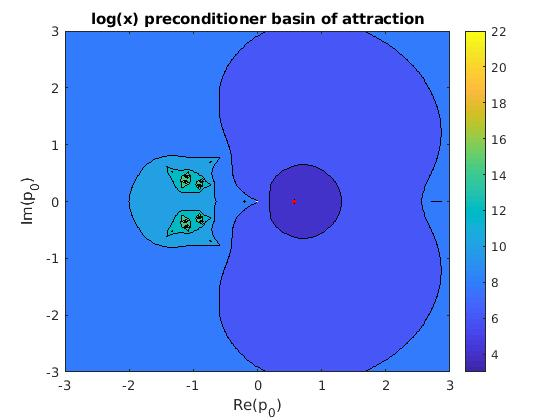
\includegraphics[width=\textwidth]{exp1_02.jpg}
	\end{subfigure}
\end{figure}

\subsection{Experiment 2}

For this experiment we examine a specific instance of Kepler's equation:
\begin{equation}
f(x) = x - 0.8 \sin(x) - \frac{2 \pi}{10} = 0.
\end{equation}

Newton's method performs adequately with this method.
Rather than try to find a simpler equation (a challenge) I will complicate the function in numerous ways to see what will make Newton's method fail.

Taking $f(x)^m$ will obviously induce a root of multiplicity $m$.
This will naturally reduce the convergence rate to linear and induce structure into the error progression.

Taking $\log(f(x) + 1)$ significantly reduced the basin of attraction for the real root.
It also allowed for imaginary roots to be found.
There were several choices of initial guess that did not converge within 100 iterations.
Interestingly, these choices led to the largest number of iterations for the normal case.
These areas correspond roughly with very low values of the derivative:
$x = \arccos(0.8) = 0.6435 + n 2 \pi$.

Taking $\exp(-1/\abs{f(x)})$ results in the iteration
\begin{equation*}
p_{n+1} = p_n - \sign(f(p_n)) f(p_n)^2 / f'(p_n) .
\end{equation*}
It is possible to get convergence with this iteration, however it is neither accurate nor efficient.
The tolerance must be lowered substantially or significantly more iterations allowed.
So far this is the worst form of the equation.

\begin{figure}
	\begin{subfigure}{0.5\textwidth}
		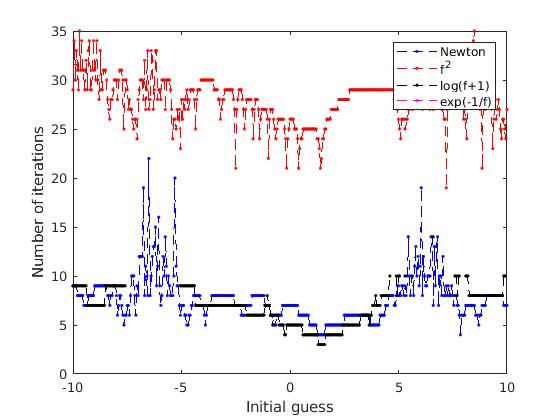
\includegraphics[width=\textwidth]{exp2_01.jpg}
	\end{subfigure}
	\begin{subfigure}{0.5\textwidth}
		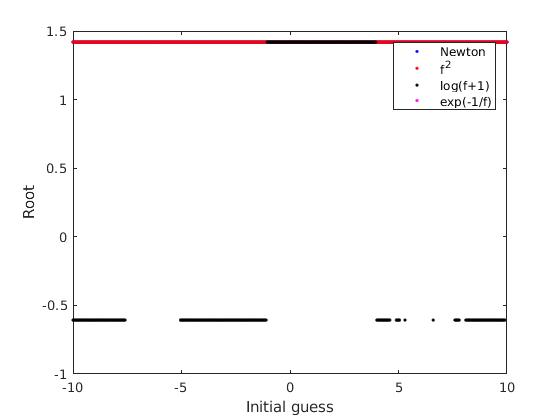
\includegraphics[width=\textwidth]{exp2_02.jpg}
	\end{subfigure}
\end{figure}

\subsection{Experiment 3}

Finally, we examine the following polynomial:
\begin{equation}
x^4 + 4 x^3 - 2 x^2 + 1 = 0.
\end{equation}

We have tried a number of fixed point iterations as preconditioners:
\begin{itemize}
\item $\pm (-4x^3 + 2x^2 - 1)^{1/4}$
\item $\pm \sqrt{ 0.5 x^4 + 2x^3 + 0.5 }$
\item $\frac{1}{2} x^3 + 2x^2 + \frac{1}{2x}$
\item $(-0.25 x^4 + 0.5 x^2 - 0.25)^{1/3}$
\end{itemize}
of which the second with a minus symbol performs 'best' for finding the real root and the fourth finds both imaginary roots with relative ease.

The leading order of each is 3/4, 2, 3 and 4/3 respectively.
I conjecture that it is ideal to have the leading order of the preconditioner be closest to 1 without going under.
In this way, the function $x - g(x)$ (where $g(x)$ is the fixed point function used as a preconditioner) will be roughly linear.
This conjecture may apply broadly: the more closely linear the function we wish to solve, the quicker we can solve it and with a wider basin of attraction.

\begin{figure}
	\begin{subfigure}{0.5\textwidth}
		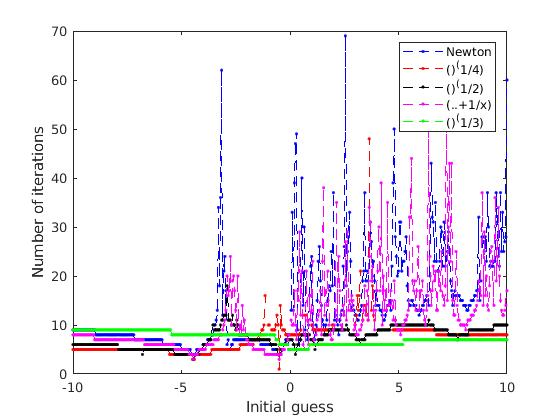
\includegraphics[width=\textwidth]{exp3_01.jpg}
	\end{subfigure}
	\begin{subfigure}{0.5\textwidth}
		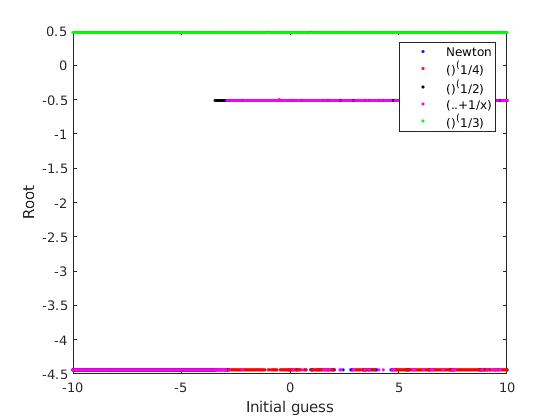
\includegraphics[width=\textwidth]{exp3_02.jpg}
	\end{subfigure}
\end{figure}

\section{Ideal preconditioning}

The best fixed point iteration we can hope for is the constant function:
\begin{equation*}
g(x) = x^*
\end{equation*}
where $x^*$ is the root we wish to converge to.
Barring this, we would like $g(x)$ to be linear, which would also guarantee single step convergence:
\begin{equation*}
g(x) = x^* + a (x - x^*) .
\end{equation*}
This last point is of interest:
the fixed point iteration will take infinite time to converge to zero, but Newton's iteration converges instantly.

It is curious that Newton's will converge in one step so long as the function is linear while a fixed point iteration will only do so if the function is constant.
It suggests a hierarchy of root finding methods, with more complicated functions converging in one step the higher up one goes.
The question is how do we go from one level of the hierarchy to another?
It seems to be something along the lines of:
\begin{equation*}
x_{n+1} = \frac{g(x) + \sum_{k=1}^n \frac{(-1)^k x_n^k g^{(k)}(x_n)}{k!}}{1 + \sum_{k=1}^n \frac{(-1)^k x_n^{k-1} g^{(k)}(x_n)}{k!} }
\end{equation*}

Failing to have knowledge of the inverse of the function we wish to find the root of, we hope that the function is, or nearly is, linear.
Failing even this, we must make compromises:
\begin{itemize}
\item if we desire greater accuracy, we require $f''(x^*)=0$, and possibly further derivatives
\item if we desire larger basins of attraction, we require $f''(x) \approx 0$ away from $x^*$
\end{itemize}

We look for a second ideal fixed point iteration.
That is, we hope to solve
\begin{equation*}
x^* = x - \frac{g(x) - x}{g'(x) - 1} .
\end{equation*}
This can be re-arranged into the following singular first order ODE:
\begin{equation*}
\begin{cases} (x - x^*) g'(x) - g(x) & = x^* \\ g(x^*) & = x^*. \end{cases}
\end{equation*}
If we make the change of variables $y = x - x^*$ and let $G(y) = g(y + x^*) - x^*$ then the ODE simplifies:
\begin{equation*}
y G'(y) - G(y) = 0
\end{equation*}
which has solution $G(y) = a y = a (x - x^*) = g(x) - x^*$, so that $g(x)$ is exactly one of the linear functions we asked for above.
Note this ODE is ill-posed: all choices of $a \in \mathbb{R}$ (and possibly $\mathbb{C}$) give solutions.

Since there already exists infinite solutions to the ODE, perhaps there is a solution of a different form.
Suppose $f(x)$ also solves the ODE, then the difference $u(x) = g(x) - f(x)$ solves the ODE
\begin{equation*}
\begin{cases} (x - x^*)u'(x) - u(x) & = 0 \\ u(x^*) & = 0. \end{cases}
\end{equation*}
This implies $u(x) = (x - x^*) u'(x)$ and $u'(x) = u'(x) + (x - x^*) u''(x)$.
It must therefore be that $u''(x) = 0$ and the only type of solutions are linear functions.
Alternatively, if we only consider the problem posed on a small domain $D$ then any solution with $u''(x) = 0 \ \forall x \in D$ will also work.

\section{Newton's method as fixed point iteration}

\begin{equation*}
z = e^{-z} = g(z)
\end{equation*}
Note for this fixed point iteration there is $2 \pi$--periodicity in the imaginary direction.
If $Re(z)>>0$ then $\abs{g(z)}<<1$.
For fixed point iterations it is important that $\abs{g'(z)}<1$.
This is true for $Re(z)>0$ so we would prefer that $Re(g(z))>0$.
This does not occur for $\abs{Im(z)}>\pi/2$ (again recall periodicity).
However, as long as $\abs{Im(g(z))}<\pi/2$ then $Re(g(g(z))>0$:
\begin{align*}
Im(g(z)) = \sin \left ( Im(z) \right ) e^{-Re(z)} .
\end{align*}

\begin{equation*}
z = g(z) = \frac{z + 1}{e^z + 1}
\end{equation*}
This is the Newton's iteration for the previous fixed point iteration.
If $Re(z)>>0$ then $\abs{g(z)}<<1$, like before.

We've established that sufficient conditions for convergence are met when $g(D) \subset D$ and $\abs{g(x)} < 1$ for all $x \in D$.
For preconditioned Newton these conditions change to:
\begin{align*}
(i) & \ x - \frac{g(x) - x}{g'(x) - 1} \in D \ \forall x \in D, \\
(ii) & \ \abs{ \frac{g''(x) (g(x) - x) }{(g'(x) - 1)^2} } < 1 \ \forall x \in D.
\end{align*}
Also included in the basin of attraction are the pre-images of these.
For fixed point iteration, $\{g^{-k}(D)\}_{k=0}^\infty$ all lie within the basin.
There is again an appropriate replacement of $g(x)$ for the same to be said of Newton's method.

\subsection{Fixed point iterations}

We examine in detail two fixed point iterations:
\begin{equation} \label{eq:FPI}
g_1(z) = e^{-z}, \quad g_2(z) = -\log(z).
\end{equation}
First and foremost, these functions have fixed points at the real root of
\begin{equation} \label{eq:f}
z e^z - 1 = 0
\end{equation}
and are inverses of each other.

The function $g_1(z)$ is $2 \pi$--periodic in the imaginary direction.
It is for this reason that it cannot converge to any of the complex roots of function \ref{eq:f}.
Likewise, this means we need only consider $-\pi \leq Im(z) < \pi$.
The function $g_2(z)$ also does not converge to complex roots by choice of branch cut.
This can be changed with the addition of $i n 2 \pi$, where $n$ is the branch cut of interest.

We are concerned with where each function will converge.
We can guarantee convergence in a region $D$ by the fixed point theorem.

\begin{thm}[Fixed point iteration theorem] \label{thm:fpi}
If a function $g(z)$ satisfies
\begin{description}
\item[(i)] $g(z) \in D$
\item[(ii)] $\abs{g'(z)} < 1$
\end{description}
for all $z \in D$ then it has a unique fixed point in $D$ and the iteration $z_{n+1} = g(z_n)$ converges to this fixed point.
\end{thm}

Consider $g_1(z)$:
condition (ii) of theorem \ref{thm:fpi} is satisfied when $Re(z) > 0$;
for condition (i) note that $g_1(z)$ rotates off the real axis by angle $-Im(z)$.
For $g_1(z)$ to satisfy $Re(g_1(z)) > 0$ it is necessary that $\abs{Im(z)} < \pi/2$.
Our region $D_0$ (the region for which $g_1(z)$ satisfies theorem \ref{thm:fpi}) is therefore:
\begin{equation} \label{eq:D1}
D_0 = \{ z \in \mathbb{C} \vert Re(z) > 0, \ -\pi/2 < Im(z) < \pi/2 \} .
\end{equation}
Given that $g_2(z)$ is the inverse of $g_1(z)$ and $D_0$ exists, there is no such region for $g_2(z)$.

\begin{figure}
	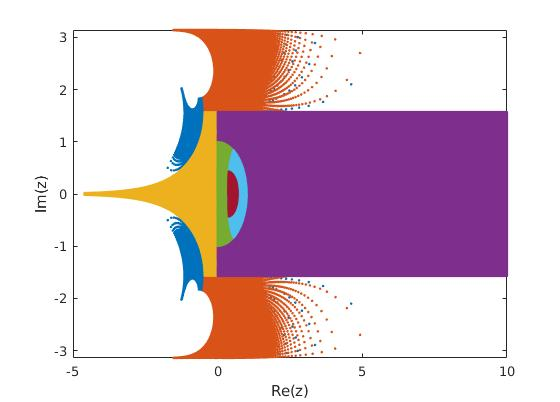
\includegraphics[width=\textwidth]{FPI_01.jpg}
	\caption{The region $D_0$ and its images under $g_1(z)$ and $g_2(z)$.}
	\label{fig:fpi01}
\end{figure}

Figure \ref{fig:fpi01} gives a representation of the region $D_0$ (purple) and its images and pre-images.
For ease of notation we define the sets $D_k$ as:
\begin{equation*}
D_{k+1} = g_1(D_k), \quad D_{k-1} = g_2(D_k).
\end{equation*}
Since $D_1 \subset D_0$ by definition of $D_0$ and $g_2(g_1(z)) = z$ there exists a hierarchy of sets:
$D_{k+1} \subset D_k \subset D_{k-1}$ for all $k \in \mathbb{Z}$.
Each set $D_{k-1}$ is the pre-image of $D_k$ under the $g_1(z)$ function.
As such, $D_{-\infty}$ represents the basin of attraction of $g_1(z)$.

\subsection{Preconditioned Newton}

We now look at applying Newton's method to the functions $g_1(z) - z$ and $g_2(z) - z$.
This will give the following fixed point iteration functions:
\begin{equation} \label{eq:Newton}
f_1(z) = \frac{z g_1'(z) - g_1(z)}{g_1'(z) - 1} = \frac{1 + z}{1 + e^z}, \quad f_2(z) = \frac{z ( 1 - \log(z) )}{1 + z} .
\end{equation}
Note that $f_1(z) = f_2(e^{-z})$ and $f_2(z) = f_1(-\log(z))$.

The function $f_1(z)$ has singularities at all branches of $\log(-1)$.
Unlike $g_1(z)$, it is not periodic in the imaginary direction.
The function $f_2(z)$ has an erroneous fixed point at $z=0$, a singularity at $z=-1$ and a root at $z = e$.
These points will be problematic and must be excluded from the basins of attraction.

We can perform the same analysis as before using theorem \ref{thm:fpi}.
Condition (ii) can be written in terms of the fixed point functions:
\begin{equation*}
\abs{f_1'(z)} = \abs{ \frac{ g_1''(z) (g_1(z) - z) }{ (g_1'(z) - 1)^2 } } < 1, \quad \abs{ \frac{ g_2''(z) (g_2(z) - z) }{ (g_2'(z) - 1)^2 } } < 1 .
\end{equation*}
This ultimately requires
\begin{equation*}
\abs{f_1'(z)} = \abs{ \frac{1 - z e^z}{(1 + e^z)^2} } < 1, \quad \abs{f_2'(z)} = \abs{ \frac{z + \log(z)}{(1 + z)^2} } < 1.
\end{equation*}

Condition (ii) holds for $f_2(z)$ except in an elliptical region containing $z=-1$.
The region where the fixed point theorem is true for $f_2(z)$, hereafter called $D_0^2$, is then the complex plane without the pre-images of this ellipse.
However, if $z \approx -1$ but not equal then $f_2(z)$ is not within this ellipse.
More precisely, the image of the ellipse is outside the ellipse.
Thus, $D_0^2$ is the entire complex plane except for the points -1, 0 and $e$ and their pre-images.
This constitutes a countable set.
(side note: the pre-image of 0 for $f_2(z)$ is $e$, so the definition of $D_0^2$ can be further simplified if desired)

Analysis for $f_1(z)$ is carried out numerically.
Through experiments we can establish that the ball of radius 1 in the complex plane represents a region where theorem \ref{thm:fpi} is satisfied.
Call this ball $D_0^1$.
We can also show that the inverse of $f_1(z)$ is
\begin{equation*}
f_1^{-1}(z) = z - 1 - W(-z e^{z-1})
\end{equation*}
where $W(z)$ is the Lambert W function (0 branch).
Using this, we repeat figure \ref{fig:fpi01}.

\begin{figure}
	\begin{subfigure}{0.5\textwidth}
		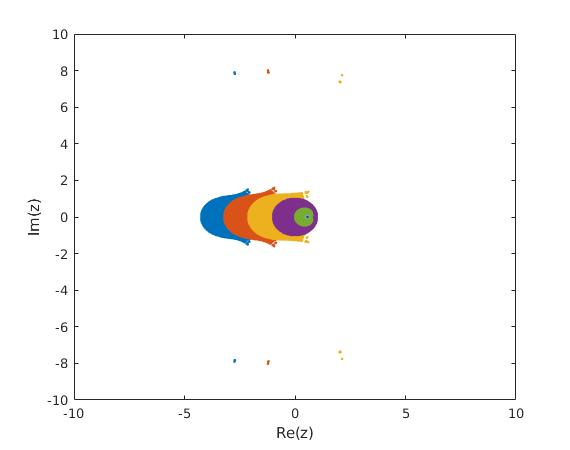
\includegraphics[width=\textwidth]{FPI_02.jpg}
		\caption{The region $D_0^1$, its images and pre-images under $f_1(z)$.}
		\label{fig:fpi02}
	\end{subfigure}
	\begin{subfigure}{0.5\textwidth}
		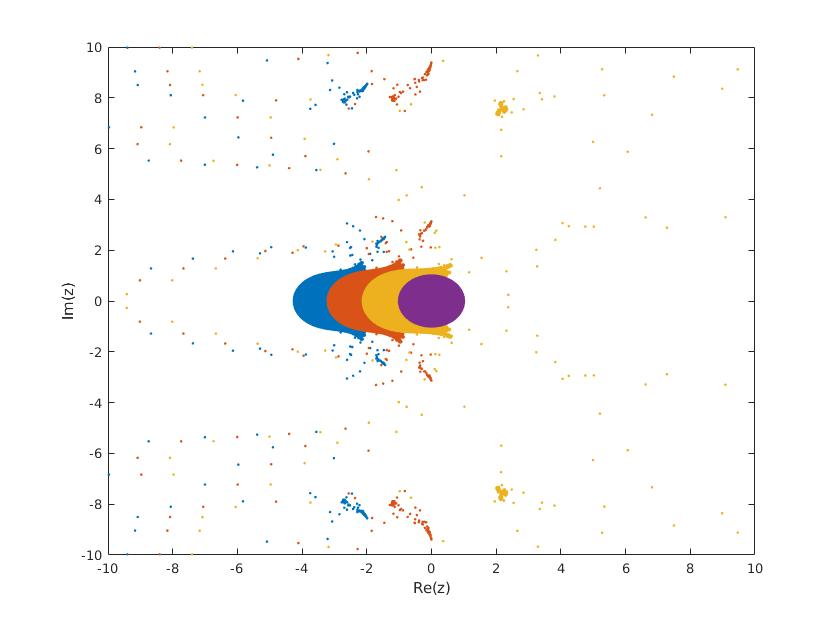
\includegraphics[width=\textwidth]{FPI_03.jpg}
		\caption{The region $D_0^1$ and its pre-images under $f_1(z)$.}
		\label{fig:fpi03}
	\end{subfigure}
\end{figure}

Figure \ref{fig:fpi02} shows the hierarchy of sets, with $D_0^1$ in purple.
Its images are inset and converge rapidly to the root.
Its pre-images extend onto the negative real line with some scattering.
A more resolved $D_0^1$ (see figure \ref{fig:fpi03}) shows greater detail in this scattering, and reveals some fractal structure.

%---New Chapter---%

\chapter{Newton's method as a time dependent PDE}

\begin{align*}
x_{n+1} & = x_n - \frac{f(x_n)}{f'(x_n)} \\
\implies \frac{x_{n+1} - x_n}{\Delta t} & = - \frac{f(x_n)}{f'(x_n)}, \ \Delta t = 1.
\end{align*}
Allowing $\Delta t$ to represent the change in some path variable $t$, the left hand side becomes an approximation to the first derivative of $x$ with respect to $t$:
\begin{align*}
\dxdy{x}{t} & = -\frac{f(x)}{f'(x)} \\
\implies \pdxdy{f}{x} \dxdy{x}{t} & = -f(x) \\
\implies \dxdy{f}{t} & = -f(x) \\
\implies f(x(t)) & = a e^{-t} .
\end{align*}

Newton's method can then be characterized as a specific choice of $g(t)$, $\Delta t$ and ODE solver in the following method:
\begin{align*}
f(x(t)) = g(t), \ \lim_{t \rightarrow T} g(t) = 0, \ 
\dxdy{x}{t} = \frac{ dg / dt }{ \partial f / \partial x } .
\end{align*}

Open questions:
\begin{itemize}
\item does the method converge? under what circumstances?
\item what makes a good choice of $g(t)$?
\item what happens when $f'(x) = 0$? is there a similar way to rewrite modified Newton's? is modified Newton's a different choice of $g(t)$?
\item it would be nice if all Newton-like methods could be brought under this umbrella, but this would be a daunting task.
\end{itemize}

The same techniques can be applied to any fixed point iteration:
\begin{align*}
x_{n+1} = g(x_n) = x_n + g(x_n) - x_n \\
\implies \dxdy{x}{t} = -x + g(x) .
\end{align*}
This makes it a perfect candidate for exponential time differencing:
\begin{align*}
x(t) = x(0) e^{-t} + e^{-t} \int_0^t g(x(s)) e^s ds, \\
x(t_{n+1}) = e^{-h} \left ( x(t_n) + \int_0^h g(x(t_n + s)) e^{s} ds \right ) .
\end{align*}

\section{Early experiments}

After some initial trials, any choice of $g(t)$ seems suitable.
Moreover, it is not necessary for $g(t)$ to be zero in the limit.
As long as $g(t)$ is zero somewhere then the method appears to converge.

The convergence seems linked to the time discretization.
Using Euler's method gives order one convergence (no surprises there).
I should test with RK4 to see if we achieve better convergence.
Note that the convergence we are interested in is global, especially for choices of $g(t)$ that are zero in finite time.

Some obvious requirements on $g(t)$:
\begin{itemize}
\item $\min f \leq \min g < \max g \leq \max f$
\item $g(t) = 0$ for some $t$ (although, if we desire a solution to $f(x) = a$ then we would require $g(t) = a$)
\end{itemize}

\section{Pathing Methods}

It no longer seems appropriate to name these methods after Newton, as they can arise on their own merit.
The main issues facing these methods are the choice of path and the time discretization.

On the issue of time discretization, obviously higher order will give more accurate results.
However, lower order discretizations can be used repeatedly to improve accuracy.
For example, Newton's method can be considered as repeated application of a pathing method using $g(t) = a (1-t)$, Euler's method and $\Delta t=1$.
Analytically, this is identical to the original derivation of Newton's method.

On the issue of the choice of path, there are a number of problems to consider.
Any features of the function must be represented in the path.
For example, we cannot use the path $g(t) = a (1-t)$ if the function has a local extrema between $p_0$ and the root, as this behaviour is not represented in the path.

For multiple roots the path will decide on which root is converged to.
For singularities, the path will need to route around into complex space, using allowable values of $f(x)$.

The most basic pathing method that appears to have great success uses $g(t) = a (1-t)$.
This arrives at a root at $t=1$.
For this path to be used, the function in question must be monotonic between the initial guess and the root.
This path cannot traverse any valleys or climb hills.

The path $g(t) = a (1-t) + i \sin(\pi t)$ was used for the example function $f(x) = 1 - 1/x$.
This path successfully routed the singularity when using an initial guess less than zero.
However, this path could not be used if $f(x)$ did not have values that allowed it to traverse this path.
For example, if the imaginary part of $f(x)$ was nowhere equal to 1 then the path would not correspond to the function, as at time $t=0.5$ we require that $f(x(0.5)) = 0.5 a + i$.

\begin{figure}
	\begin{subfigure}{0.5\textwidth}
		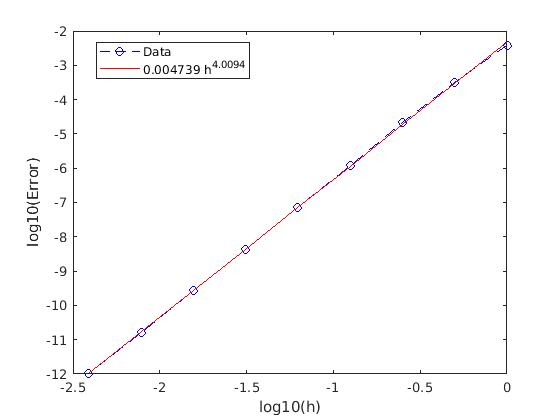
\includegraphics[width=\textwidth]{PMexp1_01.jpg}
		\caption{4th order convergence of pathing method using $g(t) = f(x_0) (1 - t)$ and RK4.}
	\end{subfigure}
	\begin{subfigure}{0.5\textwidth}
		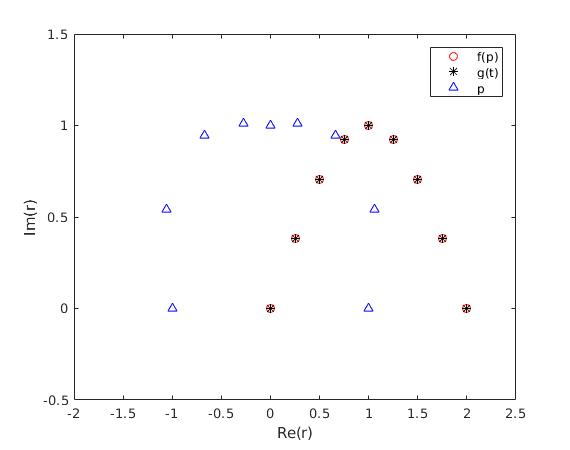
\includegraphics[width=\textwidth]{PMexp2_01.jpg}
		\caption{Path around singularity using $g(t) = f(x_0) + i \sin(\pi t)$ for $f(x) = 1 - 1/x$.}
	\end{subfigure}
\end{figure}

\section{Literature review}

%The continuous Newton method appears to originate in a paper by Airapetyan and Ramm.
%However, the Cauchy system used comes from an earlier paper by M.K. Gavurin entitled
%"Nonlinear functional equations and continuous analogies of iterative methods", published in Izu. Vuzov. Ser. Matematika 5 (1958) 18-31 (cannot find).
%As well, the paper by Airapetyan and Ramm cite two other articles that contribute in some way to CNM but none cary this identifier.
%
%On further review of the cited works, Airapetyan credits several Russian mathematicians from '58 and '67 with the genesis of CNM (Gavurin in work cited above and E.R Zhidkov and I.V. Puzynin in two articles, both from '67).
%Their work may be a bit of a challenge to track down.

\begin{description}
\item[1953] Davidenko \cite{davidenko1953new} shows the continuous analogy of Newton's method for systems (work cannot be found in English, it seems)
\item[1958] M.K. Gavurin \cite{Gavurin1958} originates the continuous analogy of Newton's method (or does he? what about Davidenko? also in Russian)
%\item[1967] Deist and Sefor "describe a novel method" involving parametrizing a system of equations and differentiating with respect to these parameters \cite{deist1967solution}
\item[1968] Galanov and Malakbovskaya provide a highly general (and uncited?) method of solving nonlinear equations \cite{galanov1968realization}
%\item[1969] Broyden describes what I believe is a continuation method \cite{broyden1969new}
\item[1972] F.H. Branin \cite{branin1972widely} suggests small change to equation (attributed to L.E. Kugel through private communication); this paper is critiqued by R.P. Brent \cite{brent1972davidenko}
\item[1975] J.P. Abbott and R.P. Brent \cite{abbott1975fast} examine convergence of the analogy (originating the term continuous Newton's method)
%\item[1978] Botsaris applies these ideas to minimization problems (possibly not first) \cite{botsaris1978differential}
%\item[1978] Chow, Mallet-Paret and Yorke assert that homotopy methods, continuation methods and continuous Newton's methods are all the same \cite{chow1978finding}
\item[1988] Saupe \cite{saupe1988discrete} has an interesting paper on several aspects of Newton's method
\item[2005] Hauser \cite{hauser2005continuous} gives an interesting discussion on the rigidity of the path $x(t)$ takes, read further
%\item[2009] Norozi et al. create a finite-time version of CNM \cite{noroozi2009finite}
\end{description}

\subsection{Some other papers of note}

\begin{description}
\item[65J15] Gibali, On the convergence rate of CNM (2016, Russian)
\item[65H05] Gutierrez, Numerical properties of different root-finding algorithms obtained for approximating CNM (2015, suggests using non-constant step sizes in time discretization)
%\item[65J15] Noroozi, Finite-time stable versions of the CNM and applications to neural networks (2009, relates method to control theory)
\item[65J15] Nair, Regularized versions of CNM and CNM under general source conditions (2008, regularization for when the inverse is not well-defined)
%\item[65K10] Zhang, A CN-type method for unconstrained optimization (200x, CNM-like method for optimization)
%\item[37F10] Jacobsen, Approximations of CNM: an extension of Cayley's problem (looks at applying several different time discretizations, very similar to Gutierrez)
\item[49M15] Neuberger, The CNM, inverse functions and Nash-Moser (basic discussions on CNM)
\item[58C15] Neuberger, Integrated form of CNM (what it says on the box)
\item[30D05] Neuberger, CNM for polynomials (examines basins of attraction for CNM on polynomials)
\item[58C15] Castro, An inverse function theorem via CNM (using CNM to prove a theorem)
\item[90C48] Attouch, The second-order in time CNM
\item[65J15] Riaza, Strong singularities and the CNM
\item[65J15] Riaza, Weak singularities and the CNM
\item[65J10] Airapetyan, CNM and its modification (convergence theorems and derivative calculations)
\item[90C30] Diener, Newton leaves and the CNM (good discussion of Branin's research and consequences, looks at extending ideas to things called Newton leaves)
\item[90C30] Diener, An extended CNM
\item[58C15] Jongen, Some reflections on the CNM for rational functions (I think this refutes some claims by Branin)
\item[65H05] Li, Path following approaches for solving nonlinear equations: homotopy, CN and projection
\end{description}

\subsection{1D test of the Davidenko-Branin method}

The Davidenko-Branin method (term coined by R.P. Brent) is a slight adjustment to the continuous Newton's method:
\begin{equation*}
\dxdy{x}{t} = \frac{ \text{adj} J}{\abs{ \det J} } f(x) .
\end{equation*}
This incorporates a sign change in the right-hand side whenever $f(x)$ passes over a 'hump'.
If CNM can be thought of as moving $f(x(t))$ along the path $f(x_0) e^{-t}$ then the DBM can be thought of as moving $f(x(t))$ along a piecewise path composed of $f(x_0) e^{-t}$ and $f(x_n) e^t$.

The overall result is that $f(x)$ is capable of surmounting 'humps' (regions of change of $f'(x)$) to continue approaching the root where Newton's method would fail.
However, this requires knowledge of where the root is with respect to starting positions.
Since $f(x)$ can now climb slopes as well as descend them towards zero, the initial sign on the right-hand side will dictate if $f(x)$ moves towards or away from the root.

We examine the function $f(x) = 0.5x + \sin(x)$ and apply a 1D version of DBM.
We achieve the results found in figure \ref{fig:DBM1} in 20 iterations of both Newton's method and DBM using Euler's method with $\Delta t = 1$.
DBM clearly has a larger basin of attraction than Newton's method.
Newton's method in particular fails outside the region of monotonicity surrounding the root.

\begin{figure}
	\begin{subfigure}{0.5\textwidth}
		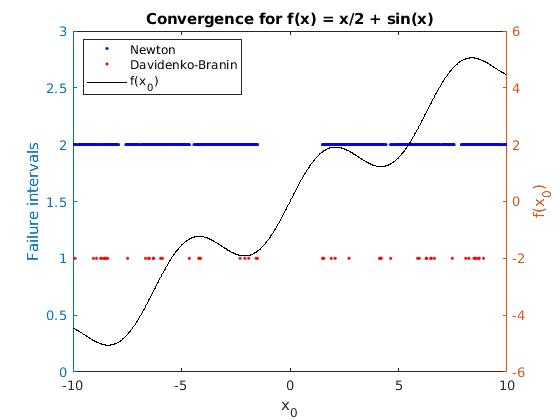
\includegraphics[width=\textwidth]{DB01.jpg}
		\caption{Initial guesses where the methods failed to converge within 20 iterations to a tolerance of $10^{-8}$.}
		\label{fig:DBM1}
	\end{subfigure}
	\begin{subfigure}{0.5\textwidth}
		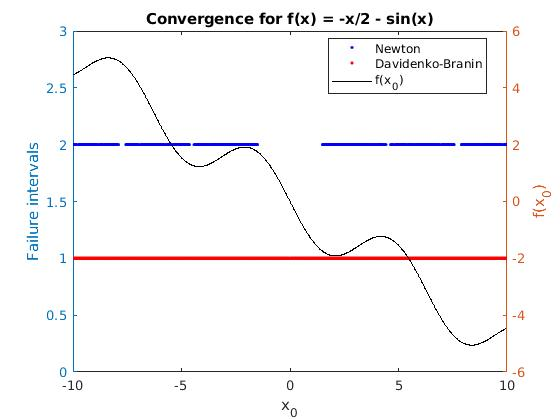
\includegraphics[width=\textwidth]{DB02.jpg}
		\caption{Initial guesses where the methods failed to converge within 20 iterations to a tolerance of $10^{-8}$.}
		\label{fig:DBM2}
	\end{subfigure}
\end{figure}

We flip the function over the real line so that the monotonicity is now reversed (figure \ref{fig:DBM2}).
DBM fails to converge for almost all points tested.
Introducing a sign change in the method will correct this.

\chapter{Schwarz methods as fixed point iterations}

Consider the alternating Schwarz method for a general second order nonlinear differential equation:
\begin{equation} \label{eq:AS}
\begin{cases} F(x,u_1^n,(u_1^n)',(u_1^n)'') = 0 & x \in [a,\beta] \\
u^n_1(a) = A \\
u^n_1(\beta) = u_2^{n-1}(\beta) \\
\end{cases}
\begin{cases} F(x,u^n_2,(u^n_2)',(u^n_2)'') = 0 & x \in [\alpha,b] \\
u^n_2(\alpha) = u^n_1(\alpha) \\
u^n_2(b) = B . \\
\end{cases}
\end{equation}
We can think of the operation to solve for $u_1^n$ as a function $G_1: \mathbb{R} \rightarrow \mathbb{R}$ such that $G_1(u_2^{n-1}(\beta)) = u_1^n(\alpha)$.
Likewise, $G_2(u_1^n(\alpha)) = u_2^n(\beta)$ and $G_2(G_1(\gamma)) = \gamma$ is a fixed point iteration.

Let $G(\gamma) = G_2 \circ G_1(\gamma)$, where $\gamma$ replaces $u^{n-1}_2(\beta)$ in equation (\ref{eq:AS}).
We will consider a single iteration and therefore drop the superscripts in the notation.
To establish how the solution of an ODE at a given point depends on the value of its endpoint, one can differentiate the ODE with respect to the endpoint:
\begin{align*}
\begin{cases} \pdxdy{F}{u} \dxdy{u_1}{\gamma} + \pdxdy{F}{u'} \dxdy{u_1'}{\gamma} + \pdxdy{F}{u''} \dxdy{u_1''}{\gamma} = 0 & x \in [a,\beta] \\
\dxdy{u_1(a)}{\gamma} = 0 \\
\dxdy{u_1(\beta)}{\gamma} = 1. \end{cases}
\end{align*}
Let $g_1(x) = \dxdy{u_1}{\gamma}$, then the ODE above may be written as:
\begin{equation*}
\begin{cases} J(u_1,u_1',u_1'') \cdot (g_1, g_1', g_1'') = 0 & x \in [a,\beta] \\ g_1(a) = 0 \\ g_1(\beta) = 1, \end{cases}
\end{equation*}
where $J(u,u',u'')$ is the Jacobian of $F(x,u,u',u'')$:
\begin{equation} \label{eq:Jacobian}
J(u,u',u'') = \left ( \pdxdy{F}{u}, \pdxdy{F}{u'}, \pdxdy{F}{u''} \right ) .
\end{equation}
Then $\dxdy{u_1(\alpha)}{\gamma} = g_1(\alpha)$.
Likewise, if $g_2(x) = \dxdy{u_2}{\gamma}$ then
\begin{equation*}
\begin{cases} J(u_2,u_2',u_2'') \cdot (g_2, g_2', g_2'') = 0 & x \in [\alpha,b] \\
g_2(\alpha) = \dxdy{u_1(\alpha)}{\gamma} = g_1(\alpha) \\ g_2(b) = 0 . \end{cases}
\end{equation*}
Therefore, $G'(\gamma) = G_2'(G_1(\gamma)) G_1'(\gamma) = g_2(\beta)$.
\begin{align*}
G'(\gamma) = \dxdy{u_2(\beta)}{\gamma} = \pdxdy{u_2(\beta)}{u_1(\alpha)} \dxdy{u_1(\alpha)}{\gamma} .
\end{align*}

There is an implicit assumption here that $G(\gamma)$ is differentiable.
If the problem is continuous with respect to the boundary data then $G(\gamma) \in C(\mathbb{R})$.
If, instead, a small perturbation in the boundary data leads to large change in the solution then we will lose the continuity of $G(\gamma)$ and most likely its differentiability.
One must then be careful when applying these methods to such problems.
Throughout this chapter we will assume $G(\gamma) \in C(\mathbb{R})$.

Note if $F(x,u,u',u'')$ is linear in $u$, $u'$ and $u''$ then $u$ depends linearly on the boundary conditions.
This is reflected in $g_1$ and $g_2$ as neither depend on $\gamma$ so long as $J(u,u',u'')$ is not explicit in its inputs.
Thus, $G''(\gamma) = 0$ for linear problems.

% rewrite this paragraph and include proofs/theorems/lemmas of its conjectures
For $G(\gamma)$ nonlinear it is possible to establish that it is a contraction mapping if the problems in $u$ and $g$ satisfy maximum and minimum principles.
If the problem in $u$ satisfies these principles for all choices of $\gamma$ then $G:\Omega \rightarrow \Omega$ where $\Omega = [ \min \{A,B\}, \max \{A,B\} ]$.
If the problem in $g$ satisfies these principles for all solutions $u_1$ and $u_2$ then we guarantee that the mapping $G(\gamma)$ contracts and that the fixed point is unique.

\begin{lemma}
If, for all $\gamma \in \mathbb{R}$, 
\begin{description}
\item[(i)] $u_1(x)$ lies between $A$ and $\gamma$ for all $x \in (a,\beta)$
\item[(ii)] $u_2(x)$ lies between $u_1(\alpha)$ and $B$ for all $x \in (\alpha, b)$
\item[(iii)] $0<g_1(x)<1$ for all $x \in (a,\beta)$
\item[(iv)] $0<g_2(x)<g_1(\alpha)$ for all $x \in (\alpha,b)$
\end{description}
then $G(\gamma)$ is a contraction mapping on $\Omega \subset \mathbb{R}$.
\end{lemma}

\begin{proof}
By the first assumption, $u_1(\alpha)$ must lie between $A$ and $\gamma$.
Thus, $u_2(\beta) \in [ \min \{A,B,\gamma\}, \max \{A,B, \gamma\} ]$ by the second assumption.
Therefore, if $\gamma \in \Omega$ then $G(\gamma) \in \Omega$.

By the third and fourth assumptions it is clear that $0 < G'(\gamma) < 1$ for all $\gamma \in \mathbb{R}$.
By the mean value theorem $\abs{G(\gamma_1) - G(\gamma_2)} \leq G'(\gamma_3) \abs{\gamma_1 - \gamma_2} < \abs{\gamma_1 - \gamma_2}$ for $\gamma_3 \in [\gamma_1, \gamma_2]$.
Thus, $G(\gamma)$ is a contraction mapping.
\end{proof}

$G(\gamma)$ is still a contraction mapping if it satisfies the assumptions for all $\gamma \in \Omega$.
Since there is a direct connection between the problems in $u$ and $g$ there is likely a connection between the assumptions on $u_1$ and $u_2$ and those on $g_1$ and $g_2$.

Applying Newton's method to $G(\gamma)$ gives the following algorithm:
\begin{equation}
\begin{aligned} \label{alg:ASPN}
(1) & \begin{cases} F(x,u_1,u_1',u_1'') = 0 \\ u_1(a) = A \\ u_1(\beta) = \gamma_n \end{cases} &
(2) & \begin{cases} F(x,u_2,u_2',u_2'') = 0 \\ u_2(\alpha) = u_1(\alpha) \\ u_2(b) = B \end{cases} \\
(3) & \begin{cases} J(u_1,u_1',u_1'') \cdot (g_1,g_1',g_1'') = 0 \\ g_1(a) = 0 \\ g_1(\beta) = 1 \end{cases} &
(4) & \begin{cases} J(u_2,u_2',u_2'') \cdot (g_2,g_2',g_2'') = 0 \\ g_2(\alpha) = g_1(\alpha) \\ g_2(b) = 0 \end{cases} \\
(5) & \gamma_{n+1} = \gamma_n - \frac{ u_2(\beta) - \gamma_n }{g_2(\beta) - 1}. & &
\end{aligned}
\end{equation}
Steps $(2)$ and $(3)$ can be performed simultaneously.
Since step $(4)$ is a linear ODE it does not necessarily require step $(3)$ as one can solve instead
\begin{equation*}
(4*) \begin{cases} J(u_2,u_2',u_2'') \cdot (g_3,\textit{g}_3',\textit{g}_3'') = 0 \\
g_3(\alpha) = 1 \\ g_3(b) = 0 \end{cases}
\end{equation*}
and use $G'(\gamma) = g_1(\alpha) g_3(\beta)$ in place of $g_2(\beta)$ in step $(5)$.

Step $(5)$ will encounter issues when approaching points where $G'(\gamma) = 1$, as this would represent an extrema of the function $G(\gamma) - \gamma$, the function to which we apply Newton-Raphson.
Assumptions (iii) and (iv) of the previous lemma give sufficient conditions that this function has no such extrema.
Later discussions will focus on alternatives when these assumptions are not valid.

Early experiments show that by adding steps 3 through 5 (straightforward linear solves) we increase convergence from linear to quadratic (see figure \ref{fig:ASPN01}).

\begin{figure}
\centering
	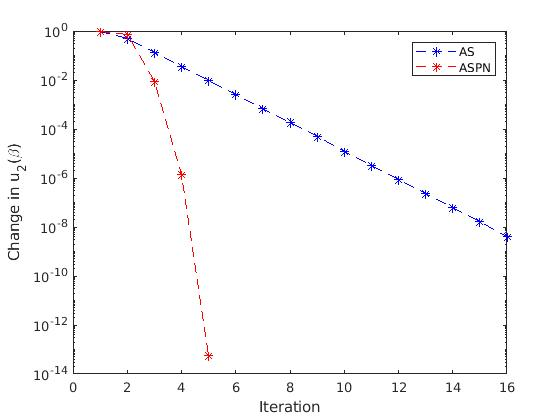
\includegraphics[width=0.5\textwidth]{ASPN01.jpg}
	\caption{Convergence rates of alternating Schwarz and the new algorithm.}
	\label{fig:ASPN01}
\end{figure}

We now look to apply this algorithm to more complicated examples.
Suppose the nonlinear function on the right hand side is also dependent on $u'$, such as in steady viscous Burgers:
\begin{equation*}
\begin{cases} \epsilon u''(x) & = u u' \\
u(-1) & = 1 \\
u(1) & = -1 . \end{cases}
\end{equation*}
Applying the algorithm we arrive at a nearly identical picture of the convergence rate as figure \ref{fig:ASPN01}.
This improvement holds for $\epsilon$ as low as $0.1$.
For smaller $\epsilon$ there is trouble finding solutions for steps $(1)$ and $(2)$.
A better nonlinear solver may be required.

Suppose one were to solve the steady viscous Burgers equation iteratively using Newton's method and domain decomposition.
This would give the following alternating Schwarz method:
\begin{align*}
(1) && u^{n+1}_1 & = u^n_1 - J(u^n_1)^{-1} f(u^n_1) , \\
(2) && u^{n+1}_2 & = u^n_2 - J(u^n_2)^{-1} f(u^n_2) , \\
&& f(u) & = \epsilon u''(x) - u(x) u'(x) .
\end{align*}
We discretize with a finite difference scheme:
\begin{equation*}
x_i = -1 + ih, \ u_i = u(x_i), \ u'(x_i) \approx \frac{u_{i+1} - u_{i-1}}{2h}, \ u''(x_i) \approx \frac{u_{i-1} - 2u_i + u_{i+1}}{h^2} .
\end{equation*}

We wish to follow the preconditioning algorithm from before.
We know there exists a fixed point iteration $G(\gamma)$ for the point $u^n_1(\beta)$.
We also know $G'(\gamma) = \pdxdy{u^n_2(\beta)}{u^n_1(\alpha)} \dxdy{u^n_1(\alpha)}{\gamma}$.
We begin by defining the problem on the first domain.

The $i$--th element of $f(u)$ on the domain $[-1,\beta]$ can be defined as:
\begin{align*}
f_i(u) & = \frac{\epsilon}{h^2} \left ( u_{i-1} - 2 u_i + u_{i+1} \right )
- \frac{u_i}{2h} \left ( u_{i+1} - u_{i-1} \right ) , \\
f_1(u) & = \frac{\epsilon}{h^2} \left ( 1 - 2 u_1 + u_2 \right )
- \frac{u_1}{2h} \left ( u_2 - 1 \right ) , \\
f_{N-1}(u) & = \frac{\epsilon}{h^2} \left ( u_{N-2} - 2 u_{N-1} + \gamma \right )
- \frac{u_{N-1}}{2h} \left ( \gamma - u_{N-2} \right ) . \\
\end{align*}
Therefore, we can define the Jacobian $J(u)$ as:
\begin{equation*}
J(u) = \begin{bmatrix} \frac{-2\epsilon}{h^2} - \frac{u_1 - 1}{2h} & \frac{\epsilon}{h^2} - \frac{u_1}{2h} & 0 & \dots & 0 \\
\frac{\epsilon}{h^2} + \frac{u_2}{2h} & \frac{-2\epsilon}{h^2} - \frac{u_3 - u_1}{2h} & \frac{\epsilon}{h^2} - \frac{u_2}{2h} & \dots & 0 \\
0 & \frac{\epsilon}{h^2} + \frac{u_3}{2h} & \frac{-2\epsilon}{h^2} - \frac{u_4 - u_2}{2h} & \dots & 0 \\
\vdots & \ddots & \ddots & \ddots & \vdots \\
0 & \dots & 0 & \frac{\epsilon}{h^2} + \frac{u_{N-1}}{2h} & \frac{-2\epsilon}{h^2} - \frac{\gamma - u_{N-2}}{2h} \end{bmatrix} .
\end{equation*}
It is then a matter of solving $J(u^n) (u^{n+1} - u^n) = -f(u^n)$ for $u^{n+1}$.

We can then calculate the derivative of $u^{n+1}$ with respect to $\gamma$ by taking such a derivative of the whole equation:
\begin{align*}
\left ( \pdxdy{J(u^n)}{\gamma} \right ) (u^{n+1} - u^n) + J(u^n) \dxdy{u^{n+1}}{\gamma} & = - \dxdy{f(u^n)}{\gamma} \\
\implies \dxdy{u^{n+1}}{\gamma} & = -J(u^n)^{-1} \left ( \left ( \pdxdy{J(u^n)}{\gamma} \right ) (u^{n+1} - u^n) + \dxdy{f(u^n)}{\gamma} \right ) \\
& = -J(u^n)^{-1} \begin{pmatrix} 0 \\ \vdots \\ 0 \\ \frac{\epsilon}{h^2} - \frac{u^{n+1}(\beta-h)}{2h} \end{pmatrix} .
\end{align*}
Note we only need the value of the derivative at the point $\alpha$.
Therefore, we pull out a single element of the matrix $J(u^n)^{-1}$:
\begin{equation*}
\dxdy{u^{n+1}_1(\alpha)}{\gamma} = \left ( \frac{u^{n+1}_1(\beta-h)}{2h} - \frac{\epsilon}{h^2} \right ) J(u^n_1)^{-1}_{\frac{\alpha+1}{h},N-1}
\end{equation*}
where $J(u^n_1)^{-1}_{i,j}$ is the element in the $i$--th row and $j$--th column of $J(u^n_1)^{-1}$.

By similar argument, we have the following formula for $\pdxdy{u^{n_1}_2(\beta)}{u^{n+1}_1(\alpha)}$:
\begin{equation*}
\pdxdy{u^{n+1}_2(\beta)}{u^{n+1}_1(\alpha)} = -\left(\frac{\epsilon}{h^2} + \frac{u^{n+1}_2(\alpha+h)}{2h} \right) J(u^n_2)^{-1}_{\frac{\beta-\alpha}{h}, 1} .
\end{equation*}
$G'(\gamma)$ is then a product of these two formulae:
\begin{equation*}
G'(\gamma) = -\left(\frac{\epsilon}{h^2} + \frac{u^{n+1}_2(\alpha+h)}{2h} \right) \left ( \frac{u^{n+1}_1(\beta-h)}{2h} - \frac{\epsilon}{h^2} \right ) J(u^n_2)^{-1}_{\frac{\beta-\alpha}{h}, 1} J(u^n_1)^{-1}_{\frac{\alpha+1}{h},N-1} .
\end{equation*}

The issue is the function $G(\gamma)$ is dependent on the initial guess $u^n$.
While we converge to the fixed point $\gamma_n$ using this iteration, the function $G(\gamma)$ is changing at each iteration.
Therefore, we have no guarantee that the Newton-Raphson iteration at step $n$ will provide an appropriate step along the function $G(\gamma)$ at step $n+1$.

We can still use this iteration by finding the fixed point of a given function $G(\gamma)$, then using this fixed point to update the solution.
That is, we run Newton's method on $G(\gamma)$, find a fixed point, then perform one iteration of Newton's method to get $u^{n+1}$.

Summary of current findings:
\begin{itemize}
\item the first algorithm described in this chapter fully solves a nonlinear system for a given transmission condition, then performs a Newton iteration to improve the transmission condition;
\item the second algorithm runs Newton's method on the transmission condition for a given $u^n$, then performs a Newton iteration to find $u^{n+1}$ using the 'best possible' transmission condition.
\item Note that the second algorithm can be made more efficient as only a rank 1 addition to the Jacobian needs to be made at each transmission condition step.
\end{itemize}

\begin{figure}
	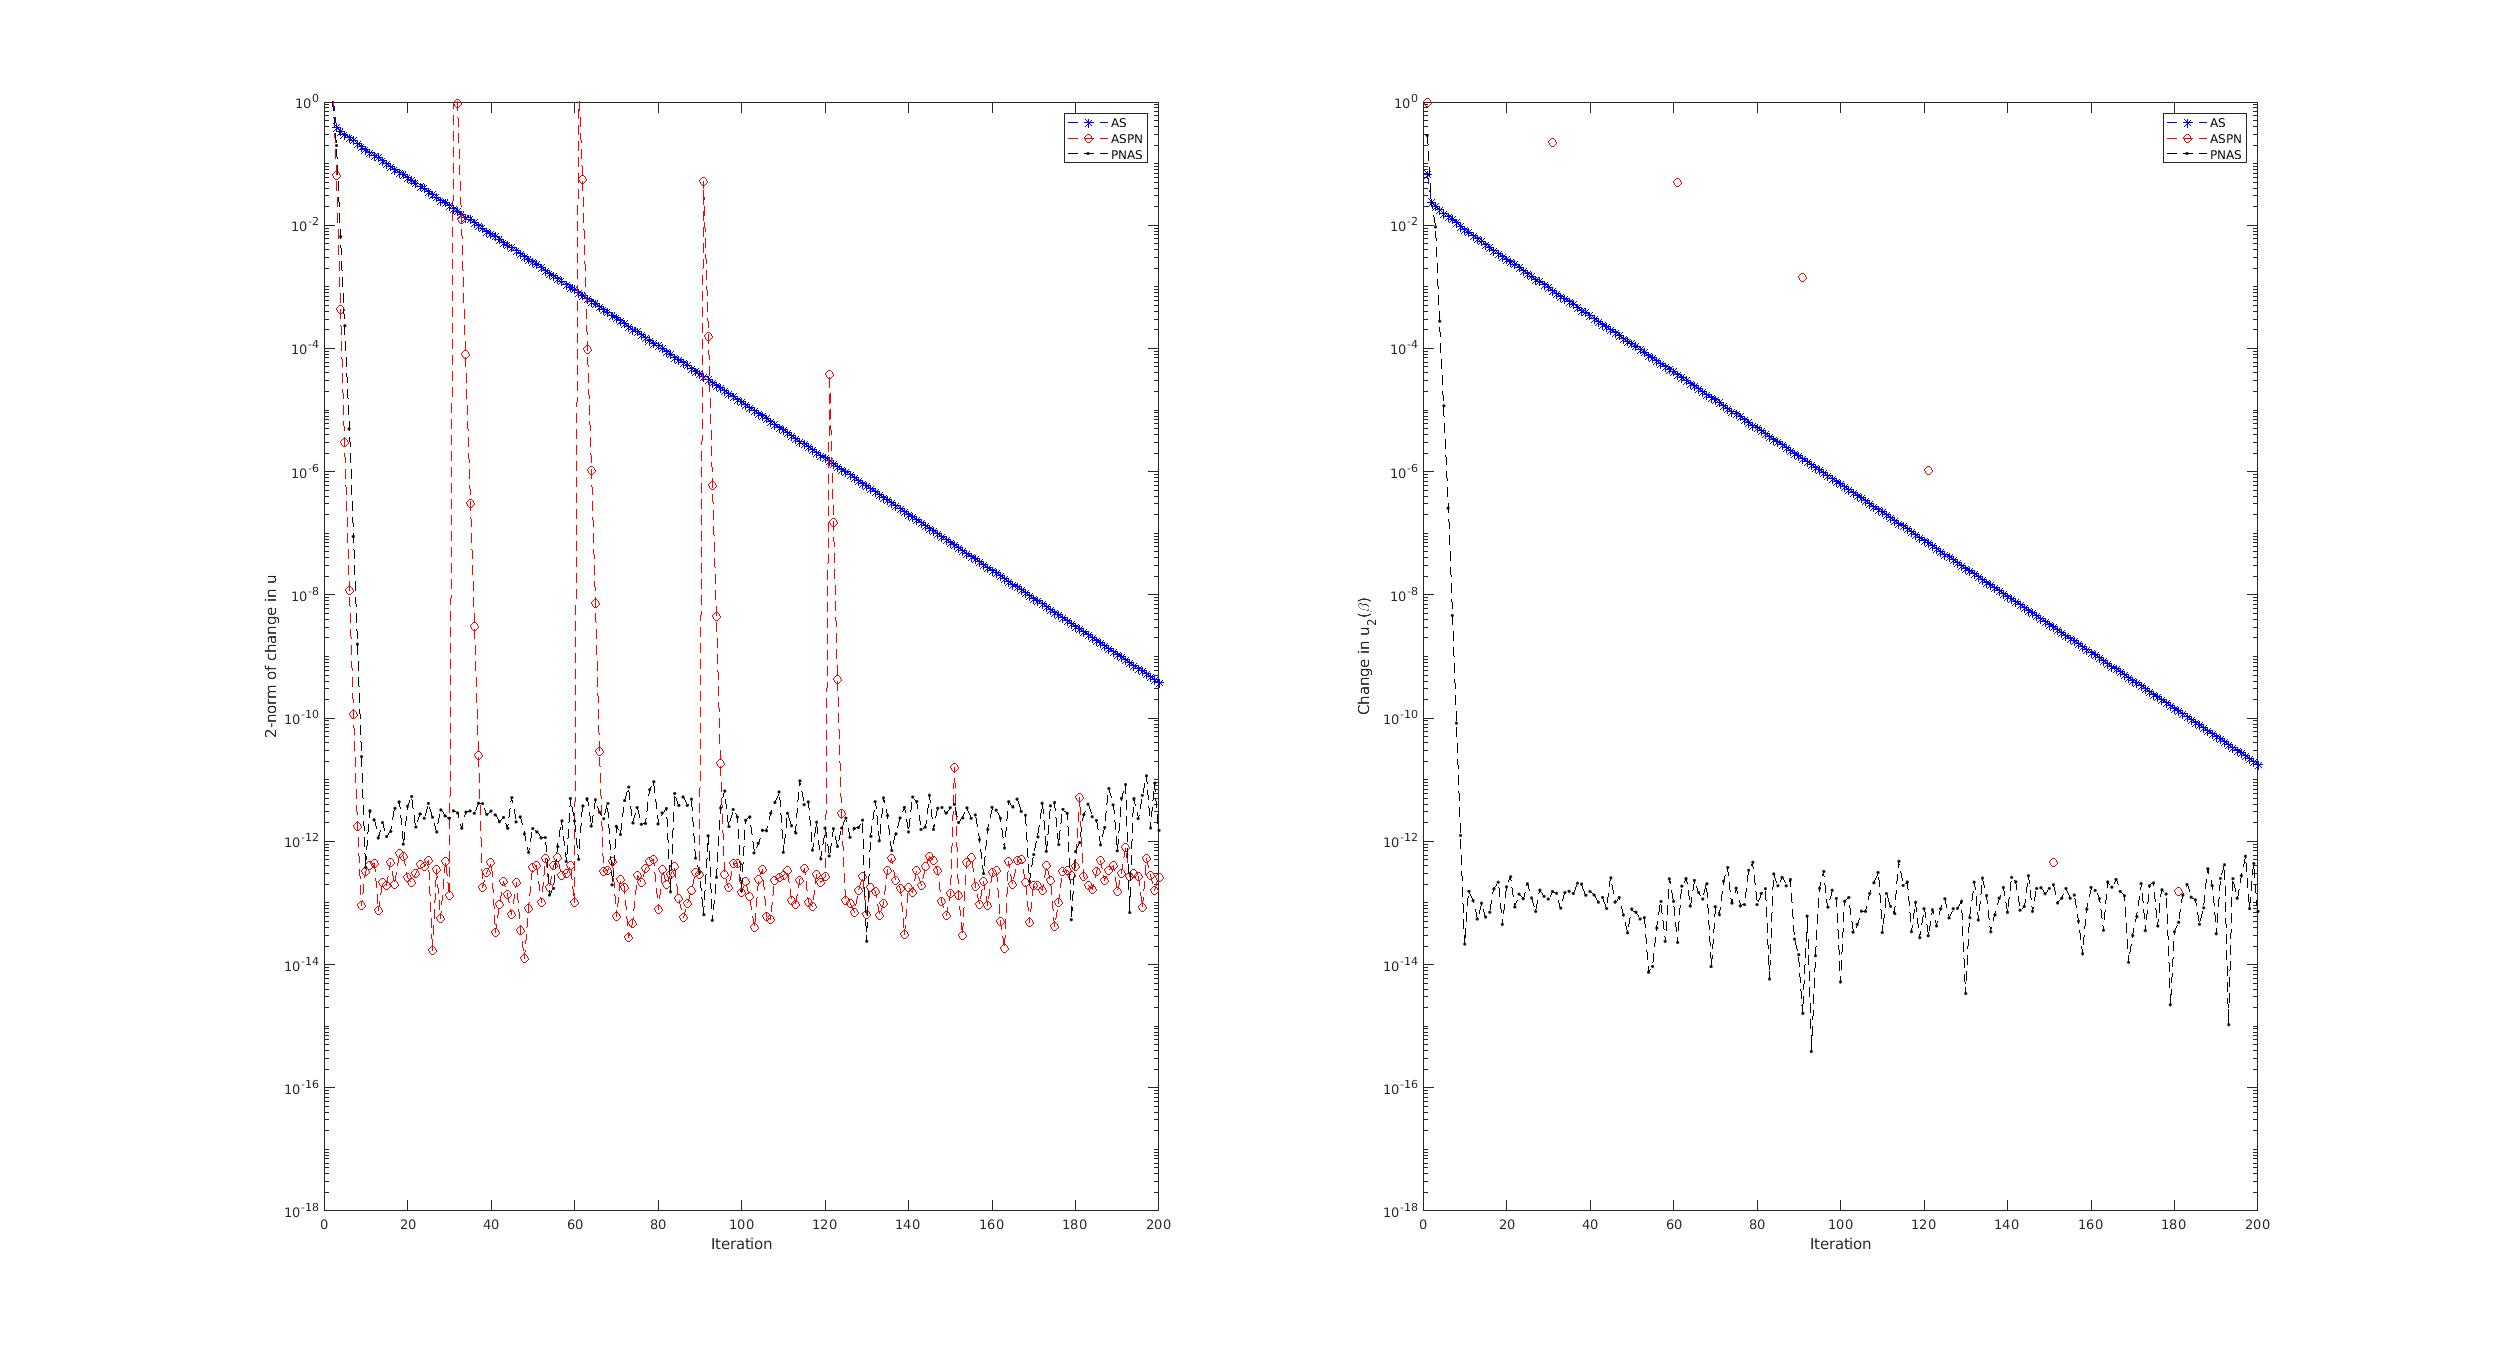
\includegraphics[width=\textwidth]{exp7_01.jpg}
	\caption{Comparison of standard additive Schwarz acting on the Newton iteration with preconditioning of the transmission condition by Newton's method both before and after an iteration of the Newton iteration on the solution. The 'iterations' along the x--axis represent roughly equal numbers of computations for all three methods. The grid used contains 1001 points, $\alpha = -\beta = -0.2$, $\epsilon = 0.1$.}
	\label{fig:ASPN}
\end{figure}

\section{Breaking the algorithms}

We seek an example for which the algorithm(s) presented in this chapter fail.
That is, we look for example problems where the Newton preconditioning on the transmission condition prevents an otherwise good alternating Schwarz iteration.
This should occur when $G'(\gamma)=1$, as this is where the function $G(\gamma)-\gamma$ has a local extrema which prevents Newton-Raphson from converging.
The algorithm would also fail if we found a cycle, but this is excluded from this analysis.
Note that $G'(\gamma) \neq 1$ if and only if $G(\gamma) - \gamma$ is monotonic, which would mean Newton-Raphson could not be expected to fail for any reasonable choice of initial guess.

We present the following theorem which, under reasonable circumstances, guarantees that the first algorithm presented in this chapter will converge for an interval surrounding the root.

\begin{thm}
Let $u(x)$ solve the second order ODE
\begin{equation*}
\begin{cases} F(u,u',u'') = 0 & x \in [a,b] \\ u(a) = A \\
u(b) = B . \end{cases}
\end{equation*}
Let $u_1(x)$, $u_2(x)$, $g_1(x)$, $g_2(x)$ be defined as in equation (\ref{alg:ASPN}) with $\gamma_n = \gamma$.
Let $G(\gamma) = u_2(\beta)$.
Let $J(x,y,z)$ be defined as in equation (\ref{eq:Jacobian}).

If $G(\gamma) \in C^1(\mathbb{R})$ and $J(u,u',u'')$ is nonsingular on both $[a,b]$ and $[\alpha,\beta]$, in the sense that the solution $v(x)$ to the ODE
\begin{equation*}
\begin{cases} J(u,u',u'') \cdot (v, v', v'') = 0 & x \in \Omega \\ v(x) = 0 & x \in \partial \Omega \end{cases}
\end{equation*}
is unique (and equal to the zero function),
then $G'(\gamma) \neq 1$ in an interval around $u(\beta)$.
As a corollary, the function $G(\gamma) - \gamma$ is monotonic in this interval.
\end{thm}

\begin{proof}
It suffices to show $G'(u(\beta)) \neq 1$.
As has been shown earlier, $G'(\gamma) = g_2(\beta)$.
Consider the difference between $g_1(x)$ and $g_2(x)$ in the region of overlap, $g(x) = g_2(x) - g_1(x)$.
This function satisfies:
\begin{equation*}
\begin{cases} J(u_2,u_2',u_2'') \cdot (g, g', g'') = \left ( J(u_2, u_2', u_2'') - J(u_1, u_1', u_1'') \right ) \cdot (g_1, g_1', g_1'') & x \in [\alpha, \beta] \\ g(\alpha) = 0 \\ g(\beta) = G'(\gamma) - 1. \end{cases}
\end{equation*}
For $\gamma = u(\beta)$ $u_1 = u_2 = u$ in the region of overlap and the right hand side is zero.
If $G'(u(\beta)) = 1$ then $g(x) = 0$ by the assumption that $J(u,u',u'')$ is nonsingular on $[\alpha,\beta]$.
Define the function $\hat{g}(x)$:
\begin{equation*}
\hat{g}(x) = \begin{cases} g_1(x) & x \in [a,\alpha] \\ g_2(x) & x \in (\alpha,b]. \end{cases}
\end{equation*}
This function satisfies:
\begin{equation*}
\begin{cases} J(u,u',u'') \cdot (\hat{g},\hat{g}',\hat{g}'') = 0 \\ \hat{g}(a) = \hat{g}(b) = 0. \end{cases}
\end{equation*}
By the assumption that $J(u,u',u'')$ is nonsingular on $[a,b]$ it must be that $\hat{g}(x) = 0$.
This contradicts $G'(u(\beta)) = 1$.
Therefore, $G'(u(\beta)) \neq 1$.
Since $G(\gamma) \in C^1(\mathbb{R})$ there is a neighbourhood of $u(\beta)$ for which $G'(\gamma) \neq 1$.
\end{proof}

The majority of uniqueness theorems on solutions to boundary value problems rely on properties satisfied by the Jacobian $J(u,u',u'')$ (nb: cite some theorems).
As such, if the problem in $u$ can be proven to have a unique solution by one of these theorems then the problem in $g$ will likewise have a unique solution, since they share a Jacobian.

If we consider instead $u_1 \neq u_2$ in the overlap region then the problem presented in the above theorem has a nonzero right hand side.
Because of this it is no longer necessary that $g(x) = 0$.
However, if $u_1$ and $u_2$ continue to converge to the same limit then the right hand side converges to zero.
The function $g(x)$ then has a magnitude related to the difference between $u_1$ and $u_2$.
%include lemma on relation, especially if J(u,u',u'') is Lipschitz

By the connection between $F()$ and $J()$ we expect that a near singularity in one problem implies the same in the other.
As such, we would expect similar instabilities in solving for $u$ as we would for $g$.
This suggests that Newton-Raphson performed on the transmission condition will always improve or maintain the convergence of the alternating Schwarz method, and any failures of the Newton-Raphson should be concomitant with failures in the alternating Schwarz.

One can use similar strategies to prove that $G(\gamma)$ is monotonic under certain conditions.
For $\alpha$ in some neighbourhood of $\beta$ this implies $G'(\gamma)>0$, as an increasing boundary condition should cause the solution nearby to likewise increase.

\begin{thm}
If the problem
\begin{equation*}
\begin{cases} F(u,u',u'') = 0 & x \in \Omega \\ u(x) = h(x) & x \in \partial \Omega \end{cases}
\end{equation*}
is nonsingular on $[a,\alpha]$ and $[\beta,b]$, in the sense that there exists a unique solution to the problem on those domains and that the continuations of these solutions are also unique, then the function $G(\gamma)$ is strictly monotonic.
\end{thm}

\begin{proof}
It suffices to show that $G(\gamma_1) = G(\gamma_2)$ implies $\gamma_1 = \gamma_2$.

Let $u^j_1$ solve the problem on $[a,\beta]$ with $u^j_1(\beta) = \gamma_j$.
Likewise, $u^j_2$ solves the problem on $[\alpha, b]$ with $u^j_2(\alpha) = u^j_1(\alpha)$.
Suppose $u^1_2(\beta) = u^2_2(\beta)$.
Then both $u^1_2$ and $u^2_2$ solve the same problem on $[\beta,b]$.
By assumption, this must mean $u^1_2 = u^2_2$ and $u^1_1(\alpha) = u^2_1(\alpha)$.
By a similar argument, this implies $u^1_1$ and $u^2_1$ solve the same problem on $[a,\alpha]$.
Again by assumption $u^1_1 = u^2_1$ and $\gamma_1 = \gamma_2$.
\end{proof}

While we are now confident that many of the problems we encounter will have $G'(\gamma) \neq 0$ we are more interested in if $G(\gamma) - \gamma$ is monotonic.
To that end, we present the following lemma, which acts as a converse to the mean value theorem for certain functions, and a corollary to this lemma giving sufficient conditions for $G'(\gamma) \neq 1$.

\begin{lemma}
If $f \in C^2([a,b])$, $f''(x) \neq 0$ for all $x \in (a,b)$ and $f'(c) = 0$ for some $c \in (a,b)$ then there exists $x_0 \in (a,b)$ such that $f(x_0)$ is equal to either $f(a)$ or $f(b)$.
Moreover, there is only one local extrema on this interval.
\end{lemma}

\begin{proof}
We begin by showing that if $f'(c_1) = f'(c_2) = 0$ then $c_1 = c_2$.
Consider the region $[c_1,c_2]$.
By the mean value theorem there must exist a point $c_3 \in (c_1,c_2)$ such that $f''(c_3) = 0$.
This contradicts the assumption that $f''(x) \neq 0$ for all $x \in (a,b)$, unless $(c_1,c_2)$ is the empty set.
Therefore, $c_1 = c_2$.

Suppose the statement is not true, that is for all $x_0 \in (a,b)$ $f(x_0) \neq f(a)$ and $f(x_0) \neq f(b)$.
Then it must be that either $f(a) < f(x_0) < f(b)$ for all $x_0 \in (a,b)$ or $f(a) > f(x_0) > f(b)$.
Then $f(x)$ is monotonic on $[a,c_1]$ and $[c_2,b]$ where $f'(c_1) = f'(c_2) = 0$.
We have already shown that $c_1 = c_2 = c$.
Thus $f(x)$ is monotonic on $[a,b]$, and $f'(x) \geq 0$ or $f'(x) \leq 0$.
WLOG we consider the former.

Let $S_1 = [a,c)$ and $S_2 = (c,b]$, and let $s_1 = \max_{x \in S_1} f'(x) > 0$ and $s_2 = \max_{x \in S_2} f'(x)) > 0$.
WLOG, $s_1 > s_2$.
Since $f'(x)$ is continuous, there exists $x_1 \in S_1$ such that $f'(x_1) = s_2 = f'(x_2)$ for some $x_2 \in S_2$.
Therefore, again by the mean value theorem, $f''(x_3) = 0$ for some $x_3 \in (x_1,x_2)$.
This contradicts the assumption that $f''(x) \neq 0$ on the interval.
Thus, it must be that the statement is true.
\end{proof}

\begin{cor}
If $G(\gamma) \in C^2(\mathbb{R})$ and $G''(\gamma^*) = 0$ implies $G(\gamma^*) = \gamma^*$ then either $G'(\gamma) \neq 1$ for all $\gamma$ or the problem is singular.
\end{cor}

\begin{proof}
Consider $f(\gamma) = G(\gamma) - \gamma$ and the domains $(-\infty,\gamma^*]$ and $[\gamma^*,\infty)$.
Apply the previous lemma to $f(\gamma)$, noting that $f(\gamma^*) = 0$ and $\liminfty{\pm \gamma} f(\gamma) = \pm \infty$.
Therefore, if $f'(\gamma_1) = 0$ for some $\gamma_1 \neq \gamma^*$ then $f(\gamma_2) = 0$ for some $\gamma_2 \neq \gamma^*$.
This implies $G(\gamma)$ has two fixed points, and therefore the problem has two solutions.
\end{proof}

These results show that, failing to have a singular problem, Newton will fail only when the second derivative of the fixed point iteration changes sign away from the root.
To this end, we present the following problem:
\begin{equation}
\label{eq:counterexample}
\begin{cases} u''(x) - \sin \left ( 15 u(x) \right ) = 0 & x \in [-1,1] \\
u(-1) = u(1) = 0 . \end{cases}
\end{equation}
The problem is uniquely solved by $u(x) = 0$.

Figure \ref{fig:exp8} shows the function $G(\gamma)$ for equation (\ref{eq:counterexample}) for $\alpha = - \beta = -0.2$ with the space between points equal to 0.01.
Also shown is the derivative $G'(\gamma)$, the function $G(\gamma) - \gamma$ and the line $y = \gamma$.
The intersection of $G(\gamma)$ and $\gamma$ represents a fixed point and a root of $G(\gamma) - \gamma$.

As can be seen in the figure, $G'(\gamma) = 1$ for some values of $\gamma$, and the derivative of $G(\gamma) - \gamma$ is zero.
Thus, Newton-Raphson applied to $G(\gamma) - \gamma$ is not guaranteed to converge.
After testing, it appears that Newton-Raphson does converge for all choices of $\gamma$ tested, albeit slowly when the initial guess is chosen near the points where $G'(\gamma) = 1$.
The importance here is the existence of a nonsingular problem for which $G'(\gamma) = 1$.

\begin{figure}
\centering
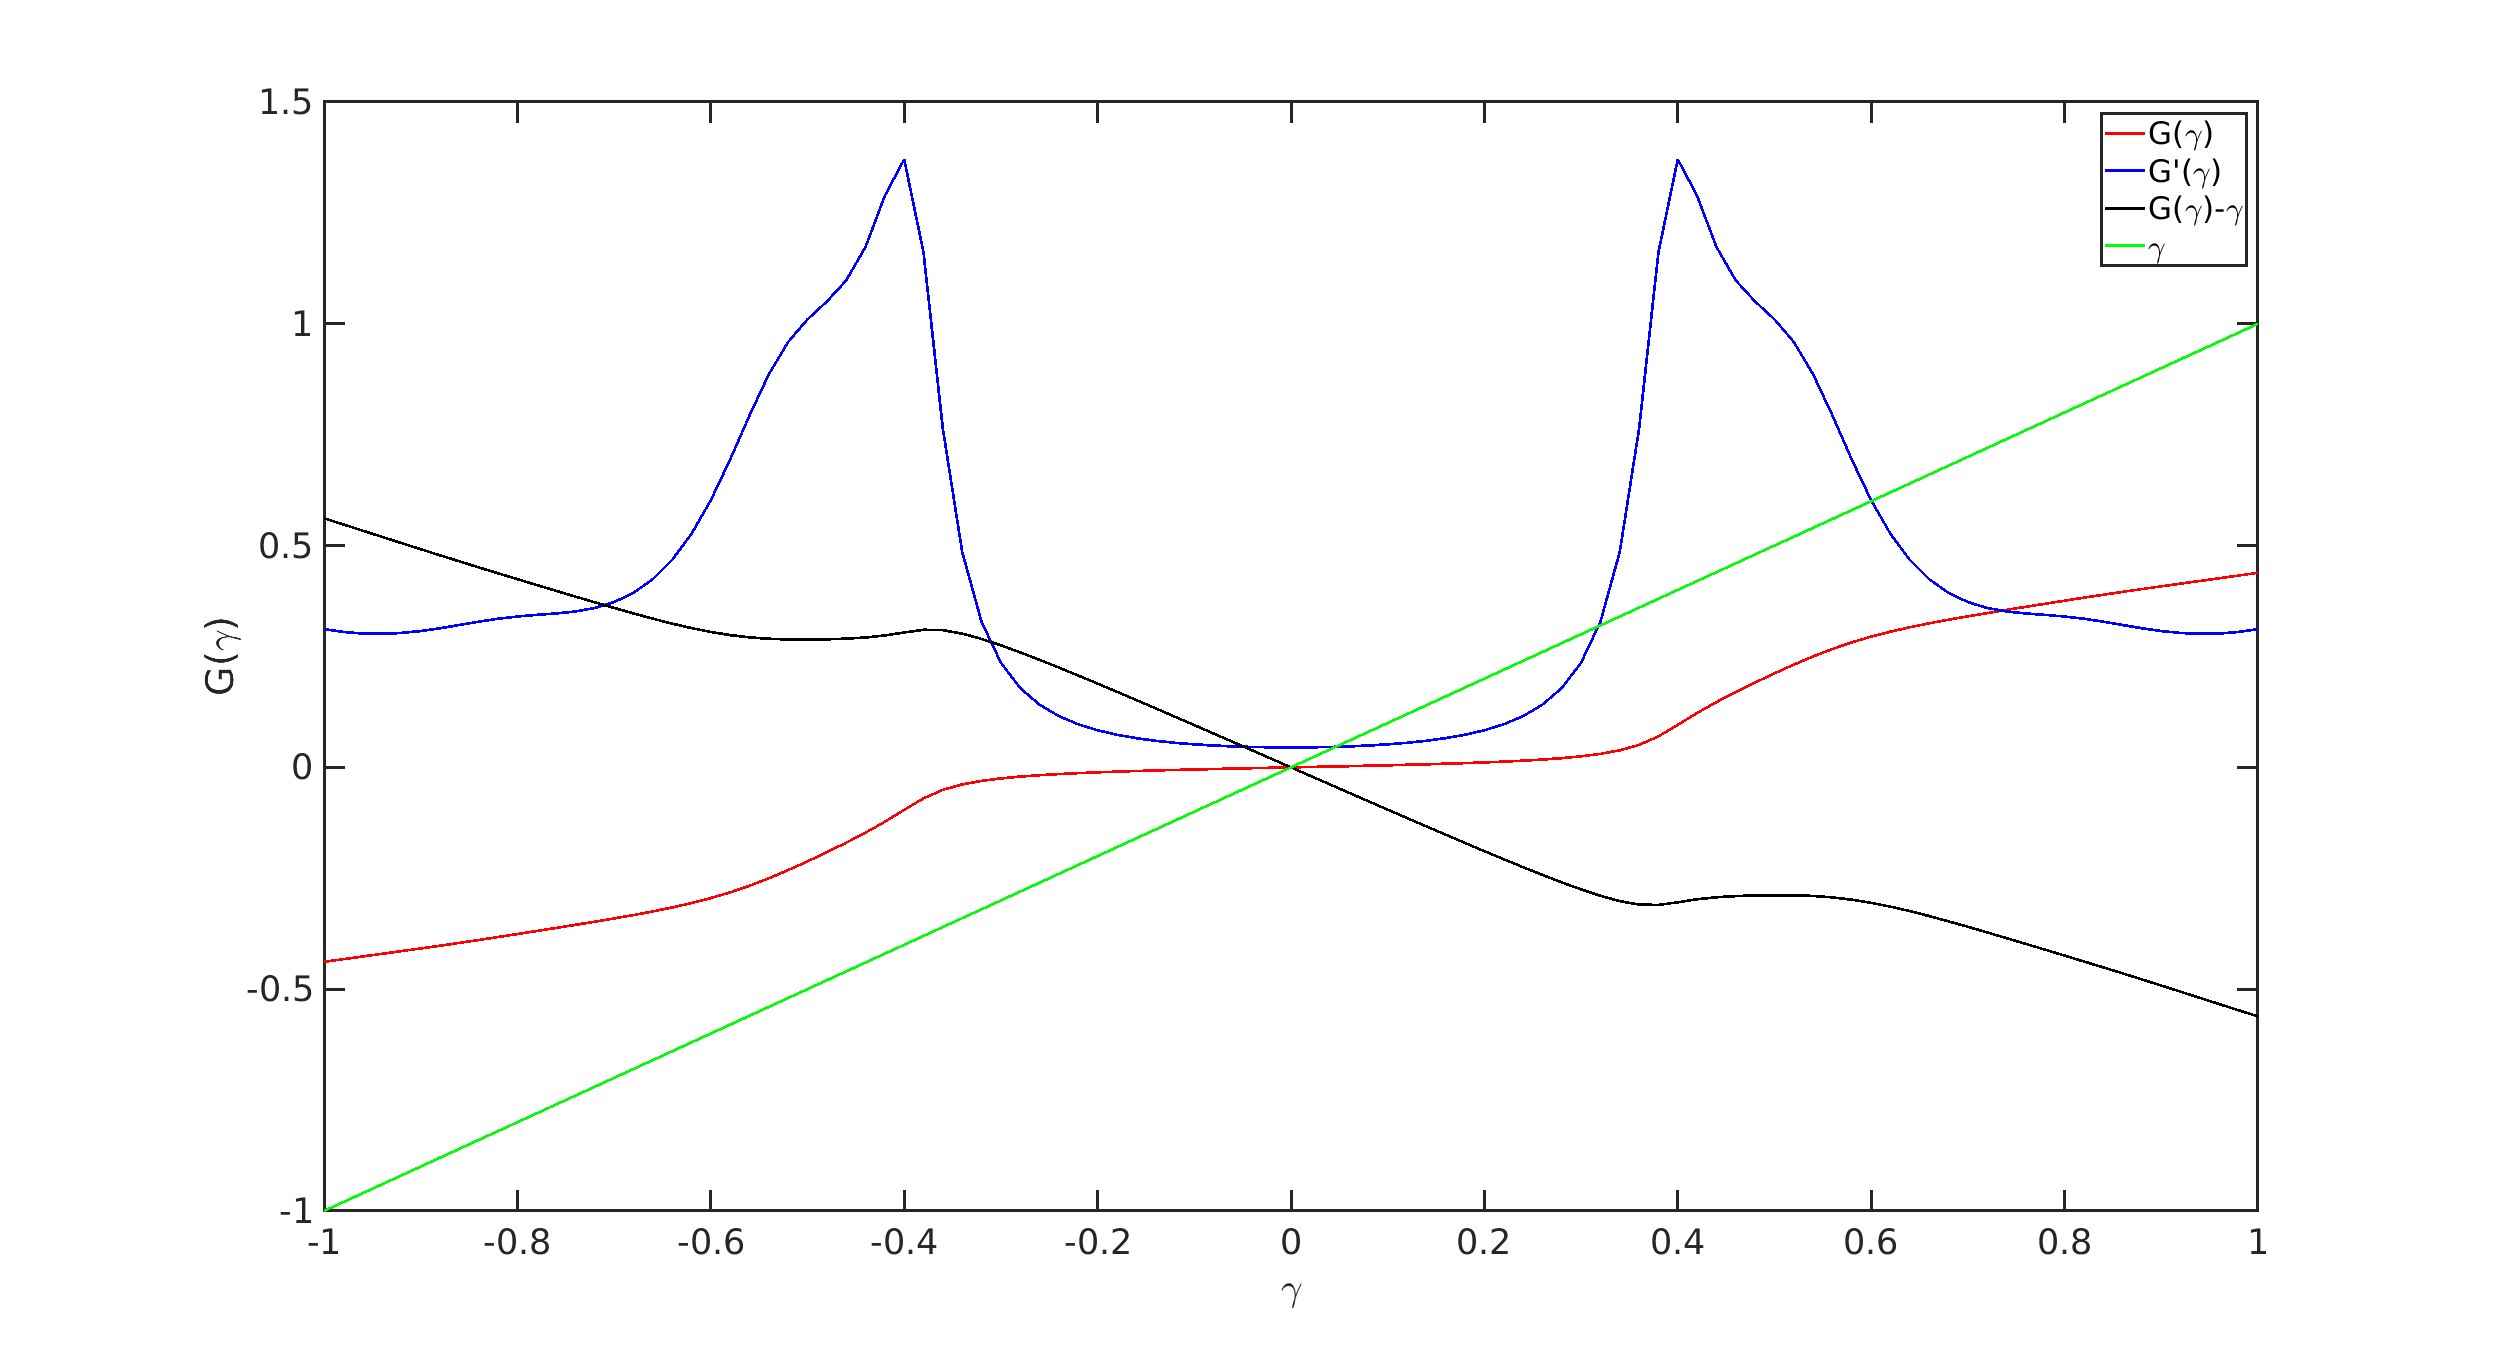
\includegraphics[width=\textwidth]{exp8_01.png}
\caption{The fixed point iterate $G(\gamma)$ and associated functions for equation (\ref{eq:counterexample}).
The point where $G(\gamma) = \gamma$ represents the fixed point.
1001 points have been used with $\alpha = -\beta = -0.2$.}
\label{fig:exp8}
\end{figure}

\section{Further analysis}

We've shown under reasonable assumptions that $G(\gamma)$ is strictly increasing.
Therefore
\begin{equation*}
\begin{cases} \gamma < G(\gamma) < \gamma^* & \gamma < \gamma^* \\
\gamma^* < G(\gamma) < \gamma & \gamma^* < \gamma . \end{cases}
\end{equation*}
We prove these conditions are sufficient for a fixed point iteration to converge.

\begin{lemma}
Let $g(x^*) = x^*$.
If $g(x) \in (x, x^*)$ for all $x \neq x^*$ then the fixed point iteration $x_{n+1} = g(x_n)$ converges towards $x^*$ for any initial guess in $\mathbb{R}$.
\end{lemma}

\begin{proof}
Since $g(x) \in (x,x^*)$, $g(x) - x^* \in (x-x^*,0)$.
Therefore, $\abs{g(x) - x^*} \in (0, \abs{x-x^*})$ and $\abs{g(x) - x^*} < \abs{x - x^*}$.
\end{proof}

As a corollary, for any value of $x$ such that $g(x) \in (x,x^*)$, $g(x)$ is closer to $x^*$ than $x$.
While this is obvious, it indicates regions of $\mathbb{R}$ for which $g(x)$ approaches its fixed point.

For a function $g(x)$ with a single fixed point there are four possible behaviours each corresponding to a quadrant of $\mathbb{R}^2$.

\begin{thm}
Let $g:\mathbb{R} \rightarrow \mathbb{R}$ and let $x^* \in \mathbb{R}$ be the only value such that $g(x^*) = x^*$.
Also let $x_{n+1} = g(x_n)$ for some $x_0 \in \mathbb{R}$ be a sequence.
\begin{description}
\item[1] If $g(x_n) < x_n < x^*$ or $x^* < x_n < g(x_n)$ then the sequence diverges monotonically.
\item[2] If $x_n < g(x_n) < x^*$ or $x^* < g(x_n) < x_n$ then the sequence converges monotonically.
\item[3] If $x_n < x^* < g(x_n) < 2 x^* - x_n$ or $2 x^* - x_n < g(x_n) < x^* < x_n$ then the sequence spirals inwards.
\item[4] If $x_n < x^* < 2 x^* - x_n < g(x_n)$ or $g(x_n) < 2 x^* - x_n < x^* < x_n$ then the sequence spirals outwards.
\end{description}
\end{thm}

\begin{proof}
All results can easily be achieved by moving the inequalities around.
\end{proof}

This shows that a fixed point iteration will converge as long as $g(x) \in (x,2x^* - x)$.
Any time that the function $g(x)$ lies within this region the fixed point iteration steps closer to the solution.
We can use this to arrive at necessary conditions on $g(x)$ for the corresponding Newton's method to converge.

\begin{description}
\item[1] $g'(x) > 1$
\item[2] $g'(x) < 1$ ($g'(x) \leq 0.5$ is sufficient)
\item[3] $g'(x) < 0.5$ ($g'(x) \leq 0$ is sufficient)
\item[4] $g'(x) < 0$
\end{description}

We examine the problem
\begin{equation*}
\begin{cases} u_{xx} = 0 & x \in [a,b] \\ u(a) = u(b) = 0 \end{cases}
\end{equation*}
with exact solution $u=0$ and Robin transmission conditions:
\begin{equation*}
u'^n_1(\beta) + C_1 u^n_1(\beta) = \gamma, \quad u'^n_2(\alpha) + C_2 u^n_2(\alpha) = u'^n_1(\alpha) + C_2 u^n_1(\alpha) .
\end{equation*}
The solutions at each step are linear functions, and so the fixed point function $G(\gamma)$ is straighforward to find:
\begin{equation*}
G(\gamma) = \gamma \frac{1 - C_1(b-\beta)}{1 + C_1(\beta-a)} \frac{1 + C_2(\alpha-a)}{1 - C_2(b - \alpha)} .
\end{equation*}

Since $G(\gamma)$ is linear, the Newton-Raphson iteration converges in a single iteration.
More interestingly, the slope $G'(\gamma)$ may take on any real value depending on the choices of $C_1$ and $C_2$.
Fixing $\alpha$ and $\beta$ and considering $G'(\gamma)$ as a function on $\mathbb{R}^2$, we have that $G':\mathbb{R}^2 \rightarrow \mathbb{R}$.

Such a function is not continuous: there are singularities along the lines $C_1 = \frac{-1}{\beta-a}$ and $C_2 = \frac{1}{b-\alpha}$.
There are also roots along the lines $C_1 = \frac{1}{b-\beta}$ and $C_2 = \frac{-1}{\alpha-a}$.
These lines also divide the boundaries between which of the four regions the fixed point iteration lies within.
While near the singularities, $G(\gamma)$ is in either region 1 or 4; while away, regions 2 or 3.
When one of the two constants is between these lines while the other is not, $G(\gamma)$ is in either region 3 or 4; if both or neither are between the lines then $G(\gamma)$ is in region 1 or 2.
%turn this into a picture?

\begin{figure}
\centering
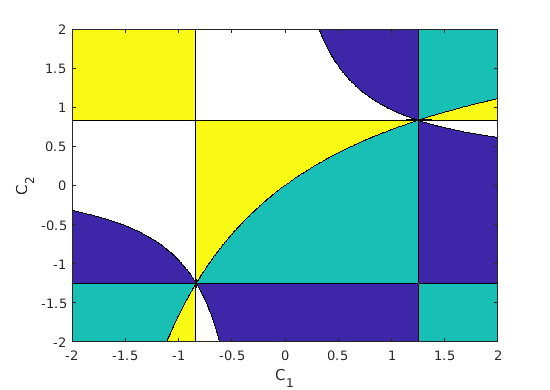
\includegraphics[width=0.7\textwidth]{exp9_01.png}
\caption{$G'(\gamma)$ as a function of $C_1$ and $C_2$ for $a = -b = -1$ and $\alpha = -\beta = -0.2$.
The regions yellow, green, blue and white correspond to the regions 1, 2, 3 and 4, respectively.}
\end{figure}

While this only applies to this particular problem, it shows that the fixed point iteration $G(\gamma)$ may appear in any of the four regions with any slope.

For a cycle to exist for the Newton-Raphson iteration, there must exist a point $x$ such that the tangent line of the fixed point function $g(x)$ at this point meets the line $y=x$ at $2 x^* - x$, where $x^*$ is the fixed point.
That is:
\begin{equation*}
g'(x) = \frac{g(x)-x^*}{2 (x-x^*)} + \frac{1}{2} .
\end{equation*}
Combined with the condition $g(x^*) = x^*$ this forms a first order ODE.
Multiplying by the integrating factor $\frac{1}{\sqrt{x-x^*}}$ and integrating we arrive at the solution:
\begin{equation*}
g(x) = x + C \sqrt{x - x^*} .
\end{equation*}
Each value of $C \in \mathbb{C}$ represents a line along which the Newton-Raphson iteration of the fixed point function $g(x)$ will be equidistant from the fixed point as the starting value.
That is, $\abs{x_0 - x^*} = \abs{x_1 - x^*}$, where $x_1$ is the application of one step of Newton-Raphson on the function $g(x)$ defined above using $x_0$ as a starting point.

The previous equation may be rewritten to isolate for the constant $C$, which may be made entirely real by introducing an absolute value sign under the radical:
\begin{equation*}
C(x) = \frac{g(x) - x}{\sqrt{\abs{x-x^*}}} .
\end{equation*}
In this way, at each point $x$ we can see which 'cycle' line the function $g(x)$ lies upon.
As long as $g(x)$ is not tangent to such a line the Newton-Raphson iteration will converge.
A sufficient condition for the convergence of Newton-Raphson is then that the function $C(x)$ defined above is strictly monotonic.
One may also use the variable $C$ as a coordinate transformation, displaying the geometry in which the function $g(x)$ must be monotonic.
This is displayed in figure \ref{fig:Clines}.
These lines may also be thought of as the pre-images of the line $2 x^* - x$ under the Newton-Raphson transformation.

\begin{figure}
\centering
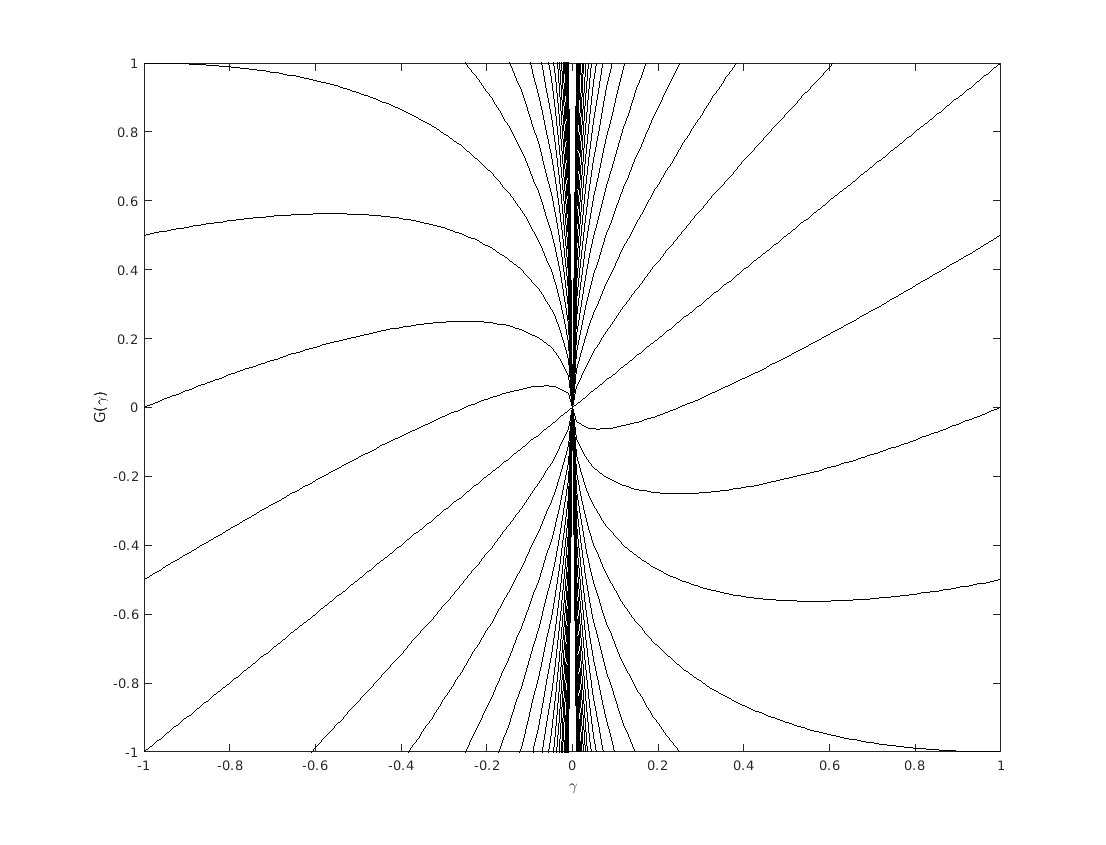
\includegraphics[width=0.7\textwidth]{clines.png}
\caption{The 'cycle' lines which represent the geometry in which $g(x)$ is ideally monotonic.}
\label{fig:Clines}
\end{figure}

While this gives some idea of the inherent geometry of the problem it is unhelpful for applications as knowledge of $x^*$ is required to calculate $C(x)$.
Note that $C(x)$ is monotonic if $g(x) > x$ and $g''(x) \geq 0$ or $g(x) < x$ and $g''(x) \leq 0$.

We can use these cycle lines to retrieve the necessary and sufficient conditions on $g(x)$ for Newton-Raphson to converge, as seen earlier, by finding where each line (denoted by $c_C(x)$) crosses the line $y=x^*$ and where its derivative is zero.
We begin with the former:
\begin{align*}
&& && x + C \sqrt{\abs{x - x^*}} & = x^* \\
&& \implies && x - x^*           & = -C \sqrt{\abs{x - x^*}} \\
&& \implies && \abs{x - x^*}^2   & = C^2 \abs{x - x^*} \\
&& \implies && \abs{x - x^*}     & = C^2 \\
&& \implies && x                 & = \begin{cases} x^* + C^2 & C < 0 \\ x^* - C^2 & C > 0. \end{cases}
\end{align*}
Therefore, the portions of $c_C(x)$ that lie within region 2 (between $x^*$ and $x$) are defined by $\abs{x - x^*} > C^2$.
Now consider the derivative of $c_C(x)$, especially for $x < x^*-C^2$ and $x > x^* + C^2$:
\begin{align*}
&& c_C'(x) & = 1 \pm \frac{C}{2 \sqrt{\abs{x-x^*}}}, \\
&& c_C'(x^* + C^2) & = 1 + \frac{C}{2 \abs{C}} \\
&&                 & = 1 - \frac{1}{2} = \frac{1}{2}, \\
&& c_C'(x^* - C^2) & = 1 - \frac{C}{2 \abs{C}} \\
&&                 & = 1 - \frac{1}{2} = \frac{1}{2}, \\
&& \lim_{x \rightarrow \pm \infty} c_C(x)  & = 1 .
\end{align*}
It is clear that $c_C''(x)$ has the same sign as $C$ for all $x \in \mathbb{R}$.
Thus, $1 \geq c_C'(x) > 1/2$ for $\abs{x - x^*} > C^2$ and if $g(x)$ lies within region 2 and $g'(x) < 1/2$ for all $x \in \mathbb{R}$ then Newton-Raphson lies within regions 2 and 3 and therefore converges.

We now consider where $c_C'(x) = 0$, so that we can find the region where if $g'(x) < 0$ then we guarantee convergence of Newton-Raphson.
We begin with $x > x^*$:
\begin{align*}
c_C'(x)  && = 1 + \frac{C}{2 \sqrt{\abs{x-x^*}}} & = 0 \\
\implies && 2 \sqrt{\abs{x-x^*}}                 & = -C & \implies C<0 \\
\implies && x                                    & = \frac{C^2}{4} + x^*, \\
         && c_C \left (\frac{C^2}{4} + x^* \right ) & = x - C \frac{C}{2} \\
&& & = x - 2 (x - x^*) \\
&& & = 2 x^* - x .
\end{align*}
We will find the same result for $x < x^*$ and $C > 0$.
Thus, in region 3 (between $x^*$ and $2 x^* - x$) $1/2 > c_C'(x) > 0$ and if $g(x)$ lies within region 3 and $g'(x) < 0$ for all $x \in \mathbb{R}$ then Newton-Raphson lies within regions 2 and 3 and therefore converges.

This analysis also shows that if $g(x)$ lies within region 1 then $g'(x) > 1$ or $C(x)$ will not be monotonic.
Likewise, if $g(x)$ lies within region 4 then $g'(x) < 0$ or $C(x)$ will not be monotonic.
These results have been summarized previously.

\bibliographystyle{plain}
\bibliography{/home/mccoid/LaTeX/references}
%\bibliography{C:/Users/conmc/Documents/LaTeX/references}

\end{document}
